\section{Small signal pump measurements}
\label{sec:small_sig_pump}

In this section the linear small signal deviation of the linearized pump model is measured and calculated.


%\subsection{One clamp push} % \label{app:...}
\subsection*{Test equipment:}
\begin{itemize}
\item The water distribution system at AAU.
\end{itemize}

\subsection*{Procedure:}
The following procedure was made for finding the small signal deviations of the pumps
\begin{enumerate}
\item Wait for the system to reach the steady state operating point.
\item Add $0.05$ to the rotational speed for one of the pumps and wait 30 minutes for steady state.
\item Note differential pressure over the pump, set the rotational speed to the operating point and 30 minutes to reach operating steady state. 
\end{enumerate}
Point 2-3 is done for each pump where the pressure over the pump is noted 

\subsection*{Measuring data:}
The data from the measurements can be seen on 

\begin{figure}[H]
% This file was created by matlab2tikz.
%
%The latest updates can be retrieved from
%  http://www.mathworks.com/matlabcentral/fileexchange/22022-matlab2tikz-matlab2tikz
%where you can also make suggestions and rate matlab2tikz.
%
\definecolor{mycolor1}{rgb}{0.00000,0.44700,0.74100}%
%
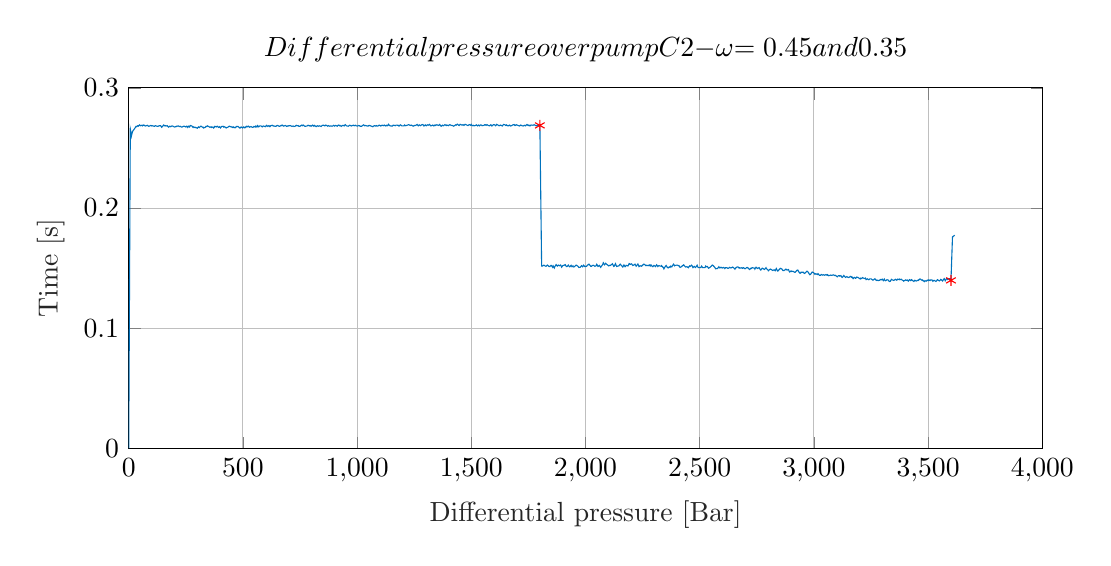
\begin{tikzpicture}

\begin{axis}[%
width=4.568in,
height=1.803in,
at={(0.753in,0.452in)},
scale only axis,
xmin=0,
xmax=4000,
xlabel style={font=\color{white!15!black}},
xlabel={Differential pressure [Bar]},
ymin=0,
ymax=0.3,
ylabel style={font=\color{white!15!black}},
ylabel={Time [s]},
axis background/.style={fill=white},
title style={font=\bfseries},
title={$\text{Differential pressure over pump C2 - }\omega\text{ = 0.45 and 0.35}$},
xmajorgrids,
ymajorgrids
]
\addplot [color=mycolor1, forget plot]
  table[row sep=crcr]{%
0	0\\
6.94999999999982	0.265744134897432\\
8.34999999999991	0.264424486803364\\
11.6999999999998	0.259817937439038\\
16.6999999999998	0.263734115347233\\
25	0.26588465298164\\
32	0.267906891495386\\
33.6999999999998	0.267613636363421\\
39.6500000000001	0.26851783968732\\
42.5	0.268163489736253\\
47.4000000000001	0.269189882697901\\
52.1999999999998	0.268487292277769\\
58.3499999999999	0.268982160312589\\
60.5	0.268450635386216\\
65.5500000000002	0.269147116324348\\
66.75	0.269043255132146\\
72.5	0.268224584555355\\
81.0999999999999	0.268841642228836\\
87.9000000000001	0.268041300097593\\
91.75	0.268261241446908\\
96.75	0.268780547409733\\
101.2	0.268304007820007\\
102.75	0.268560606060873\\
112.65	0.268016862170043\\
116.1	0.268511730205319\\
118.3	0.268475073313766\\
124.55	0.268059628543597\\
127.85	0.267980205278491\\
132.85	0.268487292277769\\
139.7	0.268468963831765\\
141.7	0.268029081134046\\
144.7	0.267222629521257\\
153.1	0.269147116324802\\
157.35	0.268389540567114\\
161	0.268615591397975\\
163	0.268200146627805\\
168.5	0.268591153470425\\
174.3	0.267277614858358\\
175	0.267350928641463\\
179.25	0.268139051808248\\
184.15	0.267674731182979\\
189.15	0.268377321603111\\
193.85	0.268132942326702\\
198.85	0.26753421309877\\
201.9	0.267436461388115\\
208.2	0.268077956989146\\
209.1	0.267845796676283\\
215.8	0.26834677419356\\
217.75	0.268358993157563\\
221.15	0.267796920821183\\
225.4	0.268035190616047\\
230.9	0.267430351906114\\
234.55	0.267479227761669\\
240.65	0.268084066471147\\
243.75	0.268114613880698\\
250	0.267479227761214\\
254.55	0.268151270771796\\
258.15	0.267155425219698\\
258.35	0.267240957966351\\
263.15	0.268139051808248\\
266.7	0.267467008797212\\
269.7	0.268731671554178\\
276.35	0.268279569892456\\
282.05	0.267100439882597\\
283.8	0.267595307917873\\
290.65	0.266929374388837\\
292.55	0.2672104105568\\
300.35	0.266458944281112\\
305.3	0.267515884652767\\
309	0.266911045943289\\
314.9	0.268151270771796\\
317.1	0.268108504398697\\
323.05	0.267295943303907\\
325	0.267369257086557\\
327.15	0.266593352883319\\
334.1	0.267051564027042\\
339.05	0.268004643206041\\
341.8	0.267845796676283\\
344.55	0.268389540566659\\
350	0.267876344085835\\
355.8	0.267192082111251\\
360.75	0.267686950146526\\
363.4	0.267033235581493\\
368.4	0.267485337243215\\
372.05	0.266568914955769\\
375.05	0.267338709677006\\
377.05	0.268029081133591\\
383.8	0.267497556207218\\
387.5	0.268096285434694\\
393.85	0.267118768328146\\
398	0.267723607038079\\
401.95	0.266691104593974\\
407.1	0.267925219940935\\
413.6	0.268059628543142\\
416.65	0.267326490713458\\
419.7	0.267680840664525\\
424.55	0.267051564027042\\
426.75	0.266636119256873\\
430.65	0.267167644183701\\
433.35	0.267130987292148\\
440.1	0.268169599217799\\
449.9	0.267381476050559\\
451.5	0.267686950146526\\
456.55	0.266904936461287\\
459.3	0.267497556207218\\
465.2	0.266764418377079\\
466.75	0.266898826979286\\
471.6	0.267833577712281\\
479.05	0.267882453567836\\
487.1	0.266477272727116\\
491.25	0.267357038123009\\
492.6	0.267497556207218\\
498.65	0.266666666666424\\
503.5	0.267540322580317\\
507.6	0.266672776148425\\
508.35	0.266672776148425\\
515.5	0.26802297165159\\
518.05	0.267479227761214\\
523.1	0.268224584554901\\
525.5	0.267913000977387\\
528.5	0.267283724339904\\
535.5	0.267821358748733\\
541.65	0.26713709677415\\
544.3	0.267130987292148\\
548.7	0.267925219940935\\
553.55	0.267381476050559\\
556.55	0.268218475072899\\
561.15	0.26738758553256\\
564.35	0.268621700879521\\
569.3	0.267546432062318\\
573.85	0.26842008797621\\
579.35	0.268352883675107\\
584.35	0.267564760507867\\
589.4	0.268291788856004\\
597.75	0.267729716519625\\
599.75	0.268151270771796\\
600	0.268077956989146\\
603.7	0.268829423264833\\
608.65	0.267919110459388\\
613.65	0.268609481915519\\
618.1	0.267766373411177\\
622.4	0.268572825024421\\
628.15	0.268878299119933\\
633.15	0.268236803518903\\
634.7	0.268432306940213\\
640.05	0.268059628543142\\
645.4	0.268047409579594\\
648.9	0.268658357771073\\
652.85	0.268701124144627\\
657.85	0.268102394916696\\
662.05	0.268090175952693\\
666.65	0.268713343108175\\
669.15	0.268554496578417\\
671.9	0.269110459432795\\
675.15	0.268627810361522\\
676.9	0.268163489735798\\
686.3	0.268688905180625\\
691.65	0.267931329422936\\
698.95	0.268542277614415\\
700.55	0.268291788856004\\
706.25	0.268658357771073\\
708.65	0.268530058650867\\
714.65	0.267955767350486\\
719.9	0.268267350928454\\
723.4	0.267882453567836\\
727.85	0.268004643206041\\
733.5	0.268884408601934\\
736.8	0.268456744867763\\
741.75	0.268664467253075\\
743.95	0.268126832844246\\
750.45	0.268035190615592\\
756.3	0.268982160312589\\
761.35	0.268468963831765\\
763.65	0.269104349950794\\
771.6	0.268004643206041\\
780.05	0.268255131964452\\
785.05	0.268914956011486\\
791.35	0.268365102639109\\
794.2	0.268695014662626\\
798.65	0.26802297165159\\
800.2	0.268310117302008\\
804.7	0.269018817204142\\
810.35	0.268181818181802\\
812.65	0.268847751710382\\
820.5	0.26775415444763\\
825	0.268297898338005\\
825.65	0.268517839686865\\
830.65	0.268090175952693\\
834.2	0.268462854349764\\
842.85	0.267882453567836\\
847.95	0.26883553274638\\
853.85	0.269018817204142\\
858	0.268346774193105\\
858.9	0.268358993157108\\
863.2	0.269018817204142\\
866.65	0.268731671554178\\
870.7	0.268126832844246\\
875.25	0.268621700879521\\
878.2	0.268102394916696\\
886.15	0.268389540566659\\
890	0.268114613880698\\
891.7	0.268157380253797\\
897.5	0.268866080156386\\
900.75	0.268187927663348\\
905.85	0.268756109481728\\
913.45	0.268157380253797\\
916.65	0.268847751710382\\
919.35	0.269092130987246\\
924.35	0.268407869012663\\
925.7	0.268701124144627\\
930.7	0.267992424242038\\
933.3	0.26837121212111\\
938.35	0.268872189637932\\
943.15	0.268389540566659\\
948.15	0.26940371456476\\
950	0.268969941348587\\
953.3	0.26839565004866\\
961.1	0.268108504399152\\
967.75	0.268957722385494\\
975	0.268267350928909\\
983.3	0.269012707722595\\
986.9	0.268505620723772\\
993.85	0.268963831867495\\
995.15	0.268523949169321\\
1001.5	0.268206256109806\\
1006.5	0.268701124145082\\
1010.25	0.268511730205773\\
1013	0.268059628544052\\
1020.1	0.268084066471602\\
1025	0.268884408602389\\
1028.6	0.269250977517459\\
1032.85	0.268450635386671\\
1037.45	0.268707233627083\\
1041.45	0.268377321603566\\
1047.35	0.268212365591808\\
1049.4	0.268536168133323\\
1050.5	0.268383431085567\\
1053.3	0.268774437927732\\
1066.65	0.267882453568291\\
1068.65	0.267674731182979\\
1075	0.26851783968732\\
1077.05	0.268542277615325\\
1082.05	0.268181818182256\\
1083.95	0.268658357771528\\
1089.4	0.268181818182256\\
1091.85	0.268383431085113\\
1096.6	0.269024926686598\\
1103.4	0.268261241446908\\
1109.25	0.268994379277046\\
1114.25	0.268560606060873\\
1119.05	0.2690371456506\\
1124	0.268352883676016\\
1128.3	0.26889051808439\\
1130.75	0.268371212121565\\
1133.3	0.268646138807526\\
1137.35	0.269715298143183\\
1141.65	0.268682795699078\\
1147.8	0.268267350928909\\
1154.85	0.268230694037811\\
1156.8	0.26884164222929\\
1159.9	0.268988269795045\\
1167.15	0.268536168133323\\
1171.05	0.269006598240594\\
1179.15	0.268884408602389\\
1183.65	0.268194037146259\\
1189.15	0.269226539589908\\
1191.85	0.269000488759048\\
1195.4	0.268456744868217\\
1203.9	0.268358993157563\\
1208.35	0.269165444770806\\
1210.15	0.268505620723772\\
1217.7	0.268774437928187\\
1225.25	0.269422043011218\\
1232.75	0.268731671554633\\
1238.2	0.269031036168599\\
1241.5	0.268530058651322\\
1245.7	0.268132942326702\\
1249.95	0.268664467253529\\
1250.45	0.268536168133323\\
1258.2	0.268951612903493\\
1262.8	0.269556451613425\\
1267.8	0.268377321603566\\
1272.25	0.26923264907191\\
1277	0.268560606060873\\
1282.4	0.269220430107907\\
1287.65	0.269544232649423\\
1292.65	0.268291788856914\\
1298.2	0.269183773216355\\
1302.75	0.268475073314221\\
1308.3	0.269287634409011\\
1311.95	0.268963831867495\\
1316.95	0.269605327468526\\
1322.6	0.268346774194015\\
1324.95	0.268426197459121\\
1331.2	0.26906158357815\\
1336.2	0.268316226784464\\
1341.4	0.269177663734354\\
1343.75	0.268719452591085\\
1348.75	0.269324291300563\\
1356.45	0.268750000000182\\
1361.4	0.269568670576973\\
1366.6	0.268255131964906\\
1368.05	0.268047409580049\\
1373.5	0.268976050831043\\
1377.55	0.268462854350219\\
1384.85	0.269422043011218\\
1390	0.268664467253529\\
1392.6	0.269128787879254\\
1400	0.268548387097326\\
1404.95	0.269360948192116\\
1408.45	0.269189882698356\\
1411.65	0.268719452590631\\
1416.65	0.268804985337738\\
1422.45	0.268139051808703\\
1426.1	0.268517839687775\\
1431.15	0.269269305963462\\
1433.8	0.269006598240594\\
1438.35	0.269825268817385\\
1446.55	0.268676686217077\\
1451.1	0.269672531769629\\
1459.45	0.268976050831043\\
1463.9	0.269415933529217\\
1467.55	0.268811094819284\\
1472.45	0.26970307917918\\
1475.15	0.269538123167422\\
1485.15	0.268640029325979\\
1490.85	0.269440371456767\\
1497.3	0.268853861192838\\
1499.5	0.269544232649423\\
1499.95	0.269391495601667\\
1504.45	0.268548387096871\\
1509.4	0.268878299120388\\
1511.95	0.268462854350219\\
1517.4	0.268597262952426\\
1522.45	0.269226539589908\\
1527.25	0.268365102639564\\
1532.1	0.269098240469702\\
1535.95	0.268365102639564\\
1540.9	0.269238758553911\\
1542.3	0.269244868035457\\
1547.3	0.268560606060873\\
1555.6	0.26886608015684\\
1558.3	0.269348729228113\\
1560.45	0.269415933529217\\
1564.75	0.268817204301286\\
1568.25	0.269415933529217\\
1574.35	0.268743890518635\\
1579.75	0.26842008797712\\
1582.7	0.269000488759048\\
1585.25	0.269293743891012\\
1590.2	0.268304007820461\\
1591.6	0.268676686217532\\
1596.6	0.269299853373013\\
1602.25	0.269275415445009\\
1606.5	0.268456744868217\\
1608.3	0.268823313783287\\
1611	0.269660312806081\\
1621.95	0.268475073314221\\
1627.65	0.269037145650145\\
1635.85	0.26829789833846\\
1640.75	0.269525904203874\\
1646.5	0.269379276637665\\
1649.45	0.268774437928187\\
1654.55	0.269244868035457\\
1656.4	0.268603372434427\\
1663.25	0.268371212121565\\
1666.5	0.268982160313044\\
1667.9	0.269079912023699\\
1672.45	0.268279569892911\\
1675.1	0.268462854350219\\
1682.95	0.269299853372559\\
1687.6	0.269470918866318\\
1690.85	0.268701124145082\\
1693.6	0.268750000000637\\
1696.65	0.269336510264111\\
1711.2	0.268285679374912\\
1715.65	0.269043255132146\\
1719.4	0.268853861192838\\
1722.85	0.268389540567568\\
1726.9	0.268291788856914\\
1732.8	0.268859970674839\\
1738.1	0.268401759531116\\
1739.9	0.269006598240594\\
1743.7	0.269544232649423\\
1748.9	0.268615591397975\\
1752.1	0.269073802541698\\
1755.5	0.268377321603566\\
1758.5	0.268517839687775\\
1761.2	0.269092130987701\\
1770.2	0.268927174975943\\
1775.25	0.269336510264111\\
1784.65	0.268407869013117\\
1791.05	0.269018817204596\\
1793	0.269049364614148\\
1799	0.268615591398429\\
1800.2	0.268804985337738\\
1807.9	0.151826735093437\\
1809.55	0.151631231672127\\
1817.85	0.152510997068021\\
1824.9	0.151661779081678\\
1827.6	0.151600684262576\\
1833.3	0.152602639296674\\
1840.8	0.151307429130611\\
1844	0.151307429130611\\
1849	0.152401026393363\\
1850.25	0.152242179863606\\
1855.8	0.150763685239781\\
1858.25	0.15189393939454\\
1863.15	0.150140518084754\\
1866.6	0.151576246334571\\
1871.25	0.15295087976574\\
1876.2	0.151783968719883\\
1880.8	0.152584310850671\\
1885.75	0.151979472141193\\
1890.9	0.15268206256178\\
1891.65	0.152553763441574\\
1895.55	0.150812561095336\\
1900.9	0.1521627565985\\
1907.75	0.152535434995571\\
1910.95	0.152981427175291\\
1915.95	0.151405180841266\\
1919.05	0.151337976540162\\
1924.45	0.152431573802914\\
1924.95	0.152150537634952\\
1930.95	0.151179130010405\\
1937.1	0.152382697947814\\
1940	0.151319648094159\\
1945.15	0.151900048876087\\
1946.3	0.151014173998647\\
1950.2	0.151063049853747\\
1958	0.152504887586019\\
1959.45	0.152572091887123\\
1966.75	0.151600684262576\\
1971.05	0.150592619746021\\
1976.6	0.15070869990268\\
1982.4	0.152034457478294\\
1987.45	0.1511546920824\\
1991.75	0.152468230694467\\
1996.3	0.151362414467712\\
2004.15	0.151460166178367\\
2008.25	0.152419354839367\\
2015	0.153366324535909\\
2016.6	0.153036412512392\\
2023.35	0.151496823069465\\
2026.75	0.15154569892502\\
2029.45	0.152223851418057\\
2035.55	0.152388807429816\\
2040.6	0.151594574780574\\
2045.2	0.151820625610981\\
2049.2	0.153207478006152\\
2054.65	0.151441837732818\\
2060.95	0.152278836755158\\
2066.25	0.150714809384681\\
2066.6	0.150800342131333\\
2074.95	0.152993646139294\\
2077.8	0.154484359726212\\
2083.45	0.152798142717984\\
2088.4	0.154044477028947\\
2091.6	0.153402981427462\\
2102.05	0.151900048876087\\
2105.9	0.152382697947814\\
2108.8	0.152272727273157\\
2118.2	0.153665689149875\\
2123.55	0.151429618768816\\
2125.65	0.151631231672127\\
2131.3	0.153732893450979\\
2133.25	0.152737047898881\\
2136.35	0.151399071359265\\
2147	0.152022238514746\\
2149.95	0.153024193548845\\
2151.9	0.153335777126358\\
2163.3	0.150953079179544\\
2166.6	0.152193304008051\\
2168.2	0.152669843597778\\
2173.25	0.151221896383959\\
2174.9	0.151478494624371\\
2177.85	0.15238269794736\\
2186	0.151869501466535\\
2190.85	0.153848973607637\\
2192.35	0.153708455523429\\
2195.45	0.15314638318705\\
2201.7	0.153598484848771\\
2206.85	0.152266617791156\\
2209.85	0.152425464321368\\
2216.65	0.153341886608814\\
2221.6	0.15167399804568\\
2229.4	0.153439638319014\\
2234.4	0.151270772239059\\
2239.1	0.152052785924297\\
2245.25	0.151606793744577\\
2249.85	0.152517106550022\\
2250.5	0.152468230694467\\
2255.7	0.153372434017911\\
2258.25	0.153152492669051\\
2264.85	0.152046676442296\\
2268	0.152517106550022\\
2273.95	0.152003910069197\\
2279	0.152694281525328\\
2283.25	0.151820625611435\\
2286.2	0.152724828934879\\
2291.6	0.15167399804568\\
2294.75	0.151234115347506\\
2299.7	0.152297165200707\\
2300.65	0.152211632454055\\
2306.1	0.15135019550371\\
2311.6	0.152773704790434\\
2316.6	0.151337976540162\\
2321.1	0.152107771261399\\
2331.05	0.151606793744122\\
2332.95	0.152028347996293\\
2333.25	0.151893939394085\\
2341.35	0.150360459433614\\
2343.25	0.149462365591717\\
2349.65	0.15152126099747\\
2353.25	0.152174975562502\\
2357.95	0.150696480939132\\
2362.05	0.150164956012304\\
2366.5	0.151099706745299\\
2370.25	0.150690371456676\\
2373.05	0.151680107527227\\
2377.6	0.151056940371745\\
2383.25	0.152822580645534\\
2385.45	0.153372434017911\\
2390.1	0.15196725317719\\
2391.6	0.152168866080501\\
2398.6	0.152504887586019\\
2402	0.152517106549567\\
2407.4	0.151985581623194\\
2409	0.15213831867095\\
2414	0.150617057673571\\
2420.85	0.151252443793055\\
2423.95	0.152046676442296\\
2424.95	0.151955034213188\\
2429.9	0.152773704790434\\
2433.25	0.151979472141193\\
2438.8	0.150953079179089\\
2444.4	0.151289100684608\\
2449.9	0.150378787879163\\
2455.65	0.151832844575438\\
2458.25	0.151466275660368\\
2464.05	0.152535434995571\\
2466.7	0.151991691105195\\
2470.8	0.150464320625815\\
2475.8	0.151484604105917\\
2480.85	0.150525415445372\\
2483.75	0.151050830890199\\
2488.75	0.152449902248918\\
2491.6	0.151075268817749\\
2493.8	0.150439882698265\\
2504.5	0.150507086999369\\
2508.25	0.151728983382327\\
2513	0.150415444770715\\
2523.4	0.150507086999369\\
2524.9	0.151313538612612\\
2526.15	0.151765640274334\\
2530.85	0.151118035191303\\
2533.6	0.151368523949714\\
2538.55	0.149963343108993\\
2541.55	0.15024437927741\\
2549.9	0.151478494623916\\
2554.9	0.152614858260222\\
2558.35	0.152223851418057\\
2566.55	0.150562072336925\\
2569.3	0.14948069403772\\
2578.6	0.149761730205682\\
2583.6	0.151136363636851\\
2588.35	0.150152737048302\\
2593.4	0.150806451613335\\
2598.85	0.150097751711201\\
2604.45	0.150604838710024\\
2608.15	0.150097751711201\\
2609.75	0.14972507331413\\
2613.3	0.150470430107816\\
2618.95	0.150360459433614\\
2622.9	0.149865591398338\\
2626.5	0.149975562072541\\
2630.6	0.15068426197513\\
2636.95	0.150152737048302\\
2644.5	0.150928641251539\\
2649.6	0.150189393939854\\
2654.25	0.149181329423755\\
2658.25	0.15031769306006\\
2658.75	0.150274926686507\\
2662.3	0.150910312805991\\
2667.65	0.151075268817749\\
2672.75	0.150018328446095\\
2674.95	0.150360459433614\\
2680	0.150054985337647\\
2684.6	0.150421554252716\\
2687.15	0.149853372434336\\
2692.1	0.150409335288714\\
2697.7	0.14952956989282\\
2700.7	0.14967619745903\\
2705.4	0.150519305963371\\
2708.95	0.150580400782474\\
2715.8	0.149358504399061\\
2717.7	0.148863636363785\\
2724.1	0.14992057673544\\
2725	0.149670087977029\\
2729.75	0.150409335288714\\
2740.55	0.149993890518545\\
2741.65	0.149279081134409\\
2746.75	0.150824780059338\\
2753.25	0.149718963832129\\
2759.9	0.150470430107816\\
2764.95	0.148845307918236\\
2767.5	0.148435972630068\\
2773.7	0.150000000000546\\
2775.15	0.149951124144991\\
2783.65	0.148900293255338\\
2790.3	0.150354349951158\\
2791.6	0.149798387097235\\
2799.9	0.148142717498104\\
2800.45	0.147898338221694\\
2807.25	0.149046920821547\\
2809.75	0.149291300097957\\
2820.2	0.148020527859899\\
2824.2	0.148613147605829\\
2826.25	0.148655913978928\\
2830.4	0.147843352884593\\
2835.3	0.149712854350128\\
2841	0.147580645161725\\
2842.6	0.147641739980827\\
2849.9	0.149321847507963\\
2850.15	0.149254643206859\\
2853.25	0.14984726295279\\
2859.35	0.149425708700619\\
2864.3	0.147965542522797\\
2869.55	0.148093841642549\\
2874.9	0.148765884653585\\
2877.6	0.149254643206859\\
2882.6	0.148411534702063\\
2888.8	0.148857526882239\\
2891.4	0.147550097751719\\
2894.1	0.146835288368038\\
2900.1	0.147745601173483\\
2902.85	0.147214076246655\\
2908.2	0.14743401759597\\
2915.1	0.146652003910276\\
2918	0.146572580645625\\
2924.9	0.148112170088552\\
2929.6	0.148490957967169\\
2933.2	0.147110215053999\\
2939.2	0.145729472141284\\
2941.75	0.145894428153042\\
2943.4	0.146652003910731\\
2953.5	0.146578690127626\\
2957.85	0.14568670576773\\
2959.75	0.145582844575074\\
2969.5	0.147519550342622\\
2974.9	0.146706989247832\\
2981.35	0.144599217986524\\
2985.15	0.144800830889835\\
2991.55	0.14664589442873\\
2993.45	0.146755865102932\\
2999.9	0.146108260019901\\
3004.45	0.144831378299386\\
3008.2	0.145381231672218\\
3015.8	0.144709188660727\\
3018.05	0.145430107526863\\
3024.45	0.143994379277046\\
3028.7	0.143982160313044\\
3032.1	0.144764173998738\\
3038.2	0.14418377321681\\
3042.05	0.144532013685875\\
3047	0.144092130987701\\
3052.85	0.144666422288083\\
3057.7	0.144141006843256\\
3059.65	0.144605327468526\\
3064.95	0.143725562072632\\
3066.9	0.14379276637419\\
3072.7	0.144263196481006\\
3077.6	0.143969941349496\\
3085.75	0.144452590420769\\
3091.55	0.143829423265288\\
3093.65	0.14406158357815\\
3099.9	0.143267350929364\\
3102	0.142821358749188\\
3108	0.143762218964184\\
3111.35	0.143792766373736\\
3112.95	0.143358993158017\\
3117.95	0.143792766373736\\
3123.5	0.142283724340814\\
3125.6	0.142558651026775\\
3130.8	0.143927174975943\\
3133.2	0.14332233626601\\
3138.8	0.142332600195914\\
3144.05	0.142992424243403\\
3149.2	0.142369257087466\\
3152.7	0.142185972629704\\
3159.4	0.143163489736708\\
3165.1	0.142357038123464\\
3166.55	0.142735826002536\\
3171.75	0.141318426197813\\
3176.65	0.142338709677915\\
3182.35	0.141550586510675\\
3183.3	0.141568914956679\\
3187.15	0.142601417400329\\
3193.95	0.14221652003971\\
3199.55	0.141312316715812\\
3203.2	0.141037390029396\\
3204.6	0.141678885630881\\
3208.55	0.141342864125818\\
3212.65	0.142179863148158\\
3216.6	0.141721652004435\\
3224.1	0.141306207234265\\
3225.45	0.14162390029378\\
3228.6	0.140469208211471\\
3233.65	0.141122922776503\\
3240.2	0.140359237537268\\
3241.55	0.140518084067025\\
3244.05	0.141055718475855\\
3250.85	0.141037390029851\\
3258.5	0.139992668622199\\
3267.15	0.141202346041609\\
3273.25	0.139784946236887\\
3276.85	0.140096529814855\\
3280.8	0.139687194526232\\
3286.45	0.13985215053799\\
3291.3	0.140566959922126\\
3294.05	0.140249266862156\\
3299.05	0.14086021505409\\
3304	0.139613880743127\\
3307.85	0.140847996090542\\
3308.2	0.140609726295679\\
3312.8	0.139510019550926\\
3318.75	0.140029325513751\\
3319.55	0.140389784946819\\
3324.85	0.14019428152551\\
3330.05	0.138929618768543\\
3334.2	0.139021260997652\\
3339.2	0.140707478005879\\
3341.95	0.140328690127262\\
3349.85	0.139809384164437\\
3357.3	0.14078690127144\\
3361.8	0.140029325513751\\
3366.3	0.140756353861434\\
3367.3	0.140414222873915\\
3374.05	0.140982404692295\\
3375.9	0.140359237536813\\
3382.35	0.140823558162538\\
3383.2	0.140518084066571\\
3391.55	0.139571114370028\\
3392.8	0.139241202346511\\
3401.55	0.140249266862611\\
3404.5	0.139882697947542\\
3408.85	0.140163734115959\\
3413.35	0.13921065493696\\
3418.75	0.140481427175018\\
3423.75	0.139638318670677\\
3427.6	0.140450879765922\\
3433.2	0.139497800586923\\
3437.7	0.138941837732546\\
3441.7	0.139949902248645\\
3447.95	0.13925953079206\\
3457.85	0.140224828935061\\
3458.25	0.1399987781042\\
3464.2	0.141055718475855\\
3466.9	0.140762463343435\\
3474.25	0.139803274682436\\
3475.35	0.140157624633957\\
3483.2	0.138813538612339\\
3486	0.139595552297578\\
3491.55	0.139173998045408\\
3496.35	0.140053763441301\\
3499.85	0.139552785924025\\
3503.2	0.140249266862611\\
3508.2	0.139668866080683\\
3510.65	0.140273704790616\\
3517.2	0.140145405669955\\
3520.85	0.139100684262758\\
3525.9	0.139888807429543\\
3534.5	0.138978494624098\\
3540.9	0.140408113392368\\
3549.55	0.139375610948264\\
3550.5	0.139522238514473\\
3555.7	0.14066471163278\\
3563.45	0.139338954057166\\
3566.55	0.140279814272162\\
3570.4	0.141306207233811\\
3574.85	0.139821603128439\\
3575.15	0.139583333333576\\
3580.7	0.141330645161815\\
3585.65	0.140530303030573\\
3589.7	0.141190127077607\\
3597.35	0.141184017595606\\
3599.55	0.139760508309337\\
3600.05	0.139766617791338\\
3606.75	0.176038611925833\\
3616.5	0.177413245357002\\
};
\addplot [color=red, draw=none, mark=asterisk, mark options={solid, red}, forget plot]
  table[row sep=crcr]{%
1800	0.268774437928187\\
};
\addplot [color=red, draw=none, mark=asterisk, mark options={solid, red}, forget plot]
  table[row sep=crcr]{%
3600	0.139839931573988\\
};
\end{axis}
\end{tikzpicture}%
\caption{Small signal measurements for pump C2.}
\label{fig:small_sig_diff_press_C2}
\end{figure}

\begin{figure}[H]
% This file was created by matlab2tikz.
%
%The latest updates can be retrieved from
%  http://www.mathworks.com/matlabcentral/fileexchange/22022-matlab2tikz-matlab2tikz
%where you can also make suggestions and rate matlab2tikz.
%
\definecolor{mycolor1}{rgb}{0.00000,0.44700,0.74100}%
%
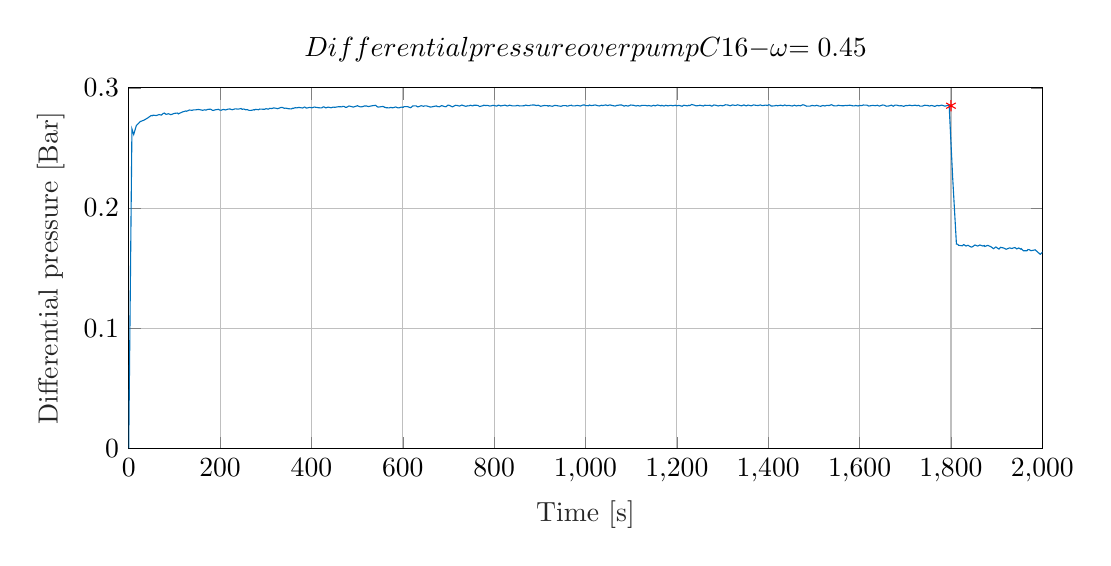
\begin{tikzpicture}

\begin{axis}[%
width=4.568in,
height=1.803in,
at={(0.766in,0.486in)},
scale only axis,
xmin=0,
xmax=2000,
xlabel style={font=\color{white!15!black}},
xlabel={Time [s]},
ymin=0,
ymax=0.3,
ylabel style={font=\color{white!15!black}},
ylabel={Differential pressure [Bar]},
axis background/.style={fill=white},
title style={font=\bfseries},
title={$\text{Differential pressure over pump C16 - }\omega\text{ = 0.45}$},
xmajorgrids,
ymajorgrids
]
\addplot [color=mycolor1, forget plot]
  table[row sep=crcr]{%
0	0\\
7.05000000000018	0.265799120234533\\
10.9499999999998	0.261223118279759\\
16.75	0.26873778103618\\
25.0999999999999	0.271939149560239\\
33.75	0.273203812316751\\
41.8000000000002	0.275012218963639\\
49.0999999999999	0.276985581622739\\
51.75	0.276759530791878\\
53.1500000000001	0.277321603128257\\
60.4000000000001	0.276979472140738\\
66.4000000000001	0.27780425219953\\
71.5500000000002	0.277352150537808\\
75.0999999999999	0.278647360703872\\
78.1999999999998	0.27905669599204\\
81.5	0.277963098729288\\
87.3499999999999	0.278470185728111\\
92.3499999999999	0.277694281524873\\
100.2	0.27881231671563\\
107.05	0.279050586510493\\
108.6	0.278341886607905\\
117	0.279863147605283\\
125	0.280816226783827\\
126.7	0.280522971651862\\
132.75	0.281567693059515\\
139	0.281292766373554\\
141.65	0.281738758553274\\
145.2	0.281641006842619\\
152.9	0.282080889540794\\
161.85	0.281329423265106\\
166.85	0.28181818181838\\
168.9	0.28144550342131\\
172.85	0.282093108504341\\
179.2	0.282306940371654\\
183.15	0.281347751710655\\
185.65	0.28122556207245\\
188.1	0.281628787878617\\
196.45	0.282178641251448\\
199.7	0.281457722385312\\
202.35	0.28142106549376\\
207.3	0.282093108504341\\
211.85	0.281641006842619\\
216.8	0.282276392962103\\
221.6	0.282459677419411\\
224.45	0.282032013685239\\
226.6	0.281836510263929\\
233.4	0.282575757575614\\
239.65	0.2823069403712\\
246.2	0.282820136852024\\
248.3	0.282166422286991\\
252.3	0.282404692081855\\
256.35	0.281732649071273\\
258.9	0.281995356793686\\
263.6	0.281256109481546\\
269.1	0.2813477517102\\
274.35	0.281860948191479\\
275.6	0.281628787878617\\
277.6	0.282166422286991\\
284.5	0.281812072335924\\
286.4	0.282386363636306\\
297.5	0.282172531768992\\
300.65	0.28267961876827\\
305.75	0.28228250244365\\
308.9	0.283003421309786\\
312.85	0.282740713587373\\
316.4	0.283247800586196\\
320.65	0.283198924731096\\
325.7	0.282685728249817\\
333.2	0.283657135874819\\
335.85	0.283767106549021\\
340.9	0.282972873900235\\
343.3	0.283168377321545\\
349.55	0.282685728249817\\
355.8	0.282478005864959\\
359.05	0.283107282501987\\
359.6	0.28289956011713\\
365.75	0.283596041055262\\
367.45	0.283327223851302\\
372.45	0.283742668621471\\
380.85	0.283266129032199\\
383.95	0.28393206256078\\
385.5	0.284054252198985\\
388.9	0.283162267839543\\
392.65	0.283431085043958\\
395.85	0.283809872922575\\
401.05	0.283418866079955\\
406.05	0.284066471162987\\
416.15	0.283455522971508\\
422.5	0.283339442814849\\
425.3	0.284078690126989\\
426.8	0.284231427174745\\
431.85	0.283339442814849\\
436.25	0.284023704789433\\
442.75	0.283455522971508\\
447.2	0.283944281524782\\
452.15	0.283864858259676\\
459.3	0.284359726294952\\
466.2	0.284219208210743\\
467.45	0.284530791788711\\
471.2	0.284585777125812\\
474.2	0.283901515151229\\
476.8	0.283815982404576\\
482.35	0.284958455522883\\
491.45	0.284042033235437\\
492.75	0.284127565982089\\
500.75	0.285135630498189\\
501.05	0.285013440859984\\
507.15	0.284219208210743\\
510.65	0.284268084066298\\
515.45	0.284897360703781\\
521.1	0.284903470185327\\
525.15	0.284426930596055\\
526.15	0.284567448680264\\
533.75	0.285184506353744\\
540.5	0.285496089931257\\
542.8	0.284659090908917\\
542.95	0.28472018572802\\
545.9	0.283974828934333\\
556.9	0.284567448680264\\
559.4	0.283999266861883\\
559.75	0.284090909090537\\
562.3	0.283534946236159\\
570.05	0.283363880742854\\
573.65	0.283779325513024\\
577.7	0.283376099706402\\
584.6	0.284133675464091\\
589.25	0.283339442814849\\
593	0.28351661779061\\
596.3	0.283962609970331\\
601.25	0.283846529814127\\
602.45	0.284365835776953\\
610.55	0.2843780547405\\
616.85	0.283479960899058\\
617.95	0.283699902247918\\
621.85	0.284946236558881\\
629.05	0.285043988269535\\
633.1	0.284139784946092\\
640.3	0.28516617790774\\
645.15	0.28469574780047\\
648.55	0.285056207233538\\
651.95	0.285007331377983\\
660.95	0.283993157379882\\
673.65	0.285019550341985\\
674.85	0.28454912023426\\
680.2	0.284274193548299\\
684.9	0.285251710654848\\
691.5	0.284463587487608\\
694.6	0.284316959921398\\
699.05	0.285691593352567\\
701.55	0.285489980449256\\
708.6	0.284200879765194\\
710.05	0.284402492668505\\
715.05	0.285496089931257\\
719.05	0.285367790811051\\
724	0.284824046920676\\
729.45	0.285716031280117\\
734.45	0.284989002932434\\
738.2	0.284659090908917\\
742.15	0.28509286412509\\
744.4	0.284989002932434\\
747.8	0.285538856304811\\
753.2	0.285007331377983\\
755.55	0.28555718475036\\
763.4	0.28548387096771\\
768.35	0.284518572824709\\
776.6	0.2852883675464\\
777.35	0.285575513196363\\
781.55	0.285251710654848\\
785	0.28548387096771\\
790.05	0.284903470185327\\
793.35	0.285025659823987\\
797.8	0.285489980449256\\
805.75	0.284811827956673\\
808.9	0.285642717497467\\
810.7	0.285496089931257\\
814.55	0.284976783968432\\
824.2	0.285679374389019\\
826.45	0.285172287389742\\
829.15	0.284976783968432\\
833.9	0.285587732159911\\
840.1	0.285007331377983\\
847.3	0.285062316715084\\
850.35	0.285441104594156\\
852.15	0.285343352883501\\
855.45	0.284958455522883\\
865.7	0.285129521016188\\
869	0.285697702834568\\
874.2	0.285178396871743\\
877.95	0.285276148582398\\
879.25	0.285630498533465\\
887.45	0.285795454545223\\
892.8	0.285276148582398\\
896.25	0.285606060605915\\
901.85	0.28469574780047\\
909.5	0.285355571847504\\
916.95	0.285184506354199\\
918.1	0.284744623656024\\
920.35	0.285227272727752\\
927.25	0.284677419355376\\
932.95	0.285465542522161\\
946.2	0.284677419355376\\
950.7	0.285270039100851\\
958	0.2852394916913\\
959.1	0.284866813294684\\
961.7	0.284860703812683\\
966.4	0.285459433040614\\
969.45	0.285526637341718\\
971.4	0.28499511241489\\
977.6	0.285074535679996\\
982.2	0.285416666667061\\
988.85	0.284903470186237\\
993.6	0.285661045943471\\
997.6	0.285874877810784\\
999.6	0.285270039100851\\
1006.4	0.285153958944647\\
1008.55	0.285728250244574\\
1012.6	0.285245601173301\\
1021.45	0.285795454545678\\
1026.45	0.285208944281749\\
1030.1	0.284952346041337\\
1035.3	0.285575513196818\\
1037.15	0.285251710655302\\
1043.4	0.285746578690578\\
1044.85	0.285740469208577\\
1048.4	0.2852394916913\\
1053.3	0.285850439882779\\
1058.25	0.285355571847958\\
1065.25	0.284848484848681\\
1068.8	0.285508308895714\\
1069.15	0.285398338221057\\
1074.85	0.285746578690578\\
1078.75	0.28580767350968\\
1084.75	0.284805718475582\\
1088.05	0.285331133920408\\
1093.05	0.284811827957128\\
1098.95	0.285746578690578\\
1105.75	0.285477761486163\\
1110.6	0.284915689149784\\
1114.25	0.285318914956406\\
1118.95	0.284879032258232\\
1122.75	0.28536168132996\\
1131.05	0.285496089931712\\
1135.3	0.28499511241489\\
1138.2	0.285367790811506\\
1144	0.284842375367134\\
1149.45	0.285508308895714\\
1152.65	0.285007331378438\\
1157.7	0.285771016618128\\
1165.35	0.285013440860439\\
1166.95	0.285483870968164\\
1171.95	0.284885141740233\\
1175.65	0.285489980450166\\
1180.65	0.285025659824441\\
1185.1	0.28541055718506\\
1187.6	0.28543499511261\\
1191.2	0.285111192571094\\
1196.75	0.285551075269268\\
1199.5	0.285050097751991\\
1204.5	0.285441104594611\\
1211.45	0.284732404692477\\
1215.3	0.285551075269268\\
1223.5	0.285001221896891\\
1226.3	0.285581622678819\\
1227.9	0.2852394916913\\
1232.35	0.286143695015198\\
1237.75	0.285654936461924\\
1242.5	0.28504398826999\\
1248.9	0.285318914956406\\
1250.2	0.285575513196818\\
1258.15	0.284909579667783\\
1261.15	0.285636608015921\\
1264.1	0.285392228739511\\
1272.65	0.285526637341718\\
1276.05	0.284836265885133\\
1277.6	0.28497067448734\\
1281.15	0.285771016618128\\
1285.95	0.285477761486163\\
1290.4	0.284946236559335\\
1295.45	0.285471652004162\\
1299.75	0.285098973607546\\
1303.25	0.285404447703058\\
1306.2	0.285929863147885\\
1311.95	0.285734359726575\\
1316.7	0.285074535679541\\
1321.75	0.285862658846781\\
1326.85	0.285392228739056\\
1329.5	0.285465542522161\\
1333.1	0.285917644183883\\
1341.65	0.28501955034244\\
1346.65	0.28583211143723\\
1351.7	0.28501955034244\\
1353.65	0.285251710655302\\
1355.9	0.285697702835023\\
1362.85	0.285074535679541\\
1368	0.285880987292785\\
1369.7	0.285673264907473\\
1377.8	0.285257820137303\\
1382.7	0.28583211143723\\
1387.05	0.285208944281749\\
1394.45	0.285685483871475\\
1398.05	0.285312805474405\\
1401.5	0.285948191593434\\
1403.05	0.28583211143723\\
1406.5	0.284891251222234\\
1413.6	0.28501955034244\\
1417.3	0.285465542522161\\
1420.4	0.285074535679541\\
1426.95	0.285630498533919\\
1432	0.285092864125545\\
1435.8	0.285734359726575\\
1437.3	0.285673264907473\\
1440.1	0.285172287390196\\
1445.1	0.285459433040614\\
1452.5	0.284909579667783\\
1457.6	0.285599951124368\\
1461.3	0.284958455523338\\
1465.8	0.285380009775508\\
1470.6	0.285092864125545\\
1475.75	0.285942082111887\\
1478.2	0.285752688172124\\
1484.3	0.284750733138026\\
1491.7	0.284860703812683\\
1496.15	0.285380009775508\\
1502.4	0.285001221896891\\
1506.3	0.285514418377716\\
1511.3	0.284891251222234\\
1514.85	0.284689638318923\\
1519.75	0.285349462365957\\
1524.1	0.284934017595788\\
1528.1	0.285477761486163\\
1533.25	0.28526392961885\\
1538.25	0.286009286412991\\
1543.2	0.285117302053095\\
1549.8	0.284982893450888\\
1553.35	0.28556329423327\\
1558.35	0.28521505376375\\
1564.9	0.285092864125545\\
1569.85	0.285477761486163\\
1571.4	0.2852394916913\\
1577.35	0.285544965787267\\
1580.45	0.285483870968164\\
1585.9	0.285007331378893\\
1589.8	0.285092864125545\\
1590.9	0.285404447703058\\
1596.7	0.284946236559335\\
1599.75	0.285380009775508\\
1604.15	0.285202834799748\\
1608.1	0.285716031281027\\
1616.1	0.285661045943471\\
1620.1	0.284879032258232\\
1629.05	0.285447214076612\\
1634.05	0.285147849462646\\
1639	0.285544965787267\\
1642.85	0.284866813294684\\
1645	0.285037878787989\\
1650.6	0.285758797654125\\
1653.65	0.285599951124368\\
1658.8	0.284744623656024\\
1664.7	0.28499511241489\\
1669.55	0.285642717497922\\
1673.75	0.284756842620027\\
1677.2	0.285569403714817\\
1680.65	0.285697702835023\\
1686.75	0.285056207233993\\
1691.9	0.285147849462646\\
1696.75	0.284640762463823\\
1701.75	0.285422776149062\\
1703.85	0.285153958944647\\
1709.6	0.28561217008837\\
1714.9	0.28516617790865\\
1721.45	0.285599951124368\\
1725.65	0.285178396872197\\
1728.85	0.285508308895714\\
1732.05	0.284836265885133\\
1737.55	0.284830156403132\\
1742.6	0.285551075269268\\
1749.65	0.285294477028856\\
1752.55	0.284909579667783\\
1757.6	0.285337243401955\\
1764.75	0.284628543499821\\
1769.7	0.285422776149062\\
1773.75	0.285025659824441\\
1779.7	0.285648826979923\\
1786.3	0.284860703812683\\
1788.6	0.284921798631785\\
1793.9	0.28558773216082\\
1796.05	0.285465542522161\\
1803.65	0.226075268817567\\
1812	0.169978005865687\\
1814.25	0.170045210166791\\
1816.65	0.16900659824114\\
1824.95	0.16861559139852\\
1827.85	0.169617546432619\\
1828.9	0.169446480938859\\
1832.85	0.168413978495209\\
1837.1	0.169018817204687\\
1844.85	0.167509775171311\\
1846.7	0.167717497556623\\
1852.5	0.169269305963553\\
1858.7	0.168395650049206\\
1863.3	0.169275415445099\\
1870.1	0.168401759531207\\
1873	0.168872189638478\\
1874.2	0.168077956989691\\
1880.6	0.168969941349587\\
1887.35	0.16787634408638\\
1893.25	0.166202346041246\\
1898.35	0.167662512219522\\
1903.7	0.166177908113696\\
1905.2	0.165927419355285\\
1908.65	0.167344819159553\\
1915.55	0.166764418377625\\
1920.8	0.165713587488426\\
1928.4	0.166904936461833\\
1933.25	0.166367302053004\\
1937.2	0.166904936461833\\
1940.1	0.167155425220244\\
1944.25	0.166012952101937\\
1948.4	0.166794965787631\\
1953.1	0.165780791789075\\
1954	0.166269550342349\\
1958.75	0.164467253177463\\
1966.8	0.164540566960113\\
1968.45	0.16548753665711\\
1971.4	0.165450879766013\\
1975.15	0.164516129032563\\
1984.25	0.165249266862702\\
1987.1	0.164235092864601\\
1987.4	0.164259530792151\\
1995.35	0.16154692082182\\
1995.75	0.161632453568473\\
2002.25	0.163899071359083\\
2007.25	0.162390029325707\\
2012.45	0.163453079179362\\
2014.55	0.162286168133051\\
2023.4	0.162939882698083\\
2029.15	0.16164467253202\\
2033.95	0.161919599218436\\
2035.3	0.160874877810784\\
2037.5	0.161589687194919\\
2040.25	0.162304496579054\\
2047.95	0.162512218963911\\
2053.65	0.160544965787267\\
2056.05	0.160361681329505\\
2061.35	0.162017350929091\\
2065.3	0.162072336266192\\
2070.25	0.161510263929813\\
2071.45	0.161754643206677\\
2076.45	0.163086510264293\\
2085.05	0.162139540567296\\
2087.6	0.161162023461202\\
2089.2	0.161522482893815\\
2091.75	0.160722140763028\\
2096.8	0.161711876833124\\
2101.85	0.160441104594611\\
2108.65	0.160819892473683\\
2113.25	0.162102883675743\\
2120.1	0.160630498534374\\
2122.85	0.161565249267369\\
2125.95	0.16073435972703\\
2131.05	0.161626344086471\\
2137.35	0.160263929619305\\
2142.55	0.161485826002718\\
2145.5	0.160007331378893\\
2150.55	0.16196236559199\\
2156.6	0.161669110460025\\
2161.75	0.160685483871475\\
2163.35	0.161553030303367\\
2166.15	0.161015395894992\\
2172.75	0.160703812317024\\
2176.4	0.161730205279127\\
2180.2	0.161412512219613\\
2185.15	0.160746578690578\\
2189.2	0.161357526882057\\
2194.05	0.160135630498644\\
2197.45	0.160826001955229\\
2200.45	0.159854594330682\\
2206.4	0.160031769306443\\
2213	0.161039833822542\\
2219.1	0.160196725318201\\
2224.3	0.160966520039437\\
2229.55	0.160276148582852\\
2233.55	0.16056329423327\\
2235.2	0.159616324536273\\
2243.25	0.16058773216082\\
2246.25	0.159225317693654\\
2248.3	0.158706011730374\\
2253.25	0.161100928641645\\
2260.05	0.15999511241489\\
2262.15	0.160935972629886\\
2267.8	0.161290322580953\\
2271.1	0.160697702835478\\
2271.55	0.16080767350968\\
2275.8	0.160483870968164\\
2280.05	0.16080767350968\\
2284.85	0.159378054740955\\
2288.8	0.160850439883234\\
2293.45	0.159396383186959\\
2299.1	0.159866813294684\\
2304.15	0.161204789834301\\
2304.7	0.160972629521439\\
2309.8	0.160141739980645\\
2316.85	0.159903470185782\\
2321.25	0.160716031280572\\
2326.55	0.160899315738334\\
2329.45	0.160392228739511\\
2331.85	0.160728250245029\\
2336.15	0.159726295210476\\
2339.3	0.160905425220335\\
2341.35	0.16036168132996\\
2348.7	0.160942082111887\\
2354.75	0.160520527859717\\
2355.35	0.16061217008837\\
2361.3	0.159787390029578\\
2363.15	0.159964565005339\\
2366.95	0.160917644184337\\
2372.5	0.159921798631785\\
2377.9	0.160905425220335\\
2382.85	0.159860703812683\\
2388.95	0.161235337243852\\
2396.55	0.159824046921131\\
2398.45	0.160398338221512\\
2405.75	0.159316959922307\\
2411.1	0.160795454546133\\
2415.05	0.160056207233993\\
2417.55	0.160801564027679\\
2422.85	0.160062316715994\\
2427.85	0.16097873900344\\
2440.8	0.160037878788444\\
2443.75	0.160667155425926\\
2447.65	0.159683528836922\\
2452.65	0.161052052786545\\
2462.8	0.160355571847958\\
2463.7	0.160581622678819\\
2467.95	0.159286412512756\\
2471.7	0.160288367546855\\
2473.85	0.161021505376993\\
2480.45	0.16100317693099\\
2483.95	0.16021505376375\\
2488.85	0.160862658846781\\
2492.05	0.160202834800202\\
2499.85	0.160636608015921\\
2503.2	0.159433040078511\\
2505.1	0.15962243401782\\
2508.05	0.160661045943925\\
2517.8	0.160764907136127\\
2521.3	0.160300586510402\\
2525.4	0.159469696969609\\
2530.15	0.160758797654125\\
2532.75	0.159976783968887\\
2539.55	0.160037878788444\\
2546.9	0.160832111437685\\
2552.35	0.1602394916913\\
2555.95	0.160746578690578\\
2563.55	0.160123411535096\\
2569.65	0.159958455523793\\
2571.6	0.160441104595066\\
2571.9	0.160398338221512\\
2578.75	0.159097018573448\\
2580.8	0.159054252199894\\
2584.45	0.160465542522616\\
2592.5	0.160673264907018\\
2595.7	0.160196725317746\\
2599.8	0.16016617790865\\
2602.5	0.160685483871475\\
2605.3	0.160502199414168\\
2608	0.160135630499099\\
2618.45	0.159524682307165\\
2621.85	0.160441104594611\\
2627.15	0.159481915934066\\
2629.5	0.160654936461469\\
2631.2	0.159811827957128\\
2637.4	0.160740469208577\\
2640	0.159811827957128\\
2645.25	0.161363636364058\\
2647.05	0.161088709678097\\
2655.4	0.159652981427826\\
2659	0.158913734115686\\
2663.75	0.159872922776231\\
2668.6	0.161064271750092\\
2672.1	0.160868768329237\\
2676.45	0.160300586510857\\
2682.75	0.160428885630608\\
2685.7	0.160844330401233\\
2693.55	0.160893206256333\\
2698.05	0.15959799609027\\
2706.8	0.161082600196096\\
2714.15	0.160147849463101\\
2719.4	0.160691593353476\\
2724.3	0.160208944282203\\
2730.75	0.160862658847236\\
2735.9	0.160025659824441\\
2738.9	0.160606060606369\\
2747.9	0.15999511241489\\
2753.25	0.160862658846781\\
2760.35	0.159982893450888\\
2763.1	0.160654936461924\\
2764.55	0.160777126100129\\
2768.95	0.159628543499821\\
2774.15	0.160801564027679\\
2779.75	0.159127565982999\\
2781.35	0.160031769306443\\
2784.65	0.160997067448989\\
2789.45	0.16075879765458\\
2794.2	0.159903470186237\\
2804.05	0.159781280548032\\
2804.85	0.160606060606369\\
2809.1	0.160917644183883\\
2813.5	0.160343352883956\\
2816.55	0.160893206256787\\
2821.75	0.159720185728929\\
2823.95	0.159652981427826\\
2829.25	0.160935972629886\\
2830.75	0.160819892473683\\
2836.6	0.159280303030755\\
2839.75	0.159090909091447\\
2847.85	0.160935972629886\\
2852.4	0.160343352883956\\
2855.95	0.160673264907473\\
2860.15	0.160227272727298\\
2868.5	0.160013440860439\\
2870.35	0.160868768328783\\
2873.55	0.160740469208577\\
2878.4	0.159628543499821\\
2881.85	0.159891251222689\\
2883.35	0.160819892473683\\
2890.65	0.160086754643544\\
2895.55	0.16100317693099\\
2898.15	0.161009286412991\\
2904.85	0.160526637341263\\
2905.95	0.160862658846781\\
2907.75	0.160098973607546\\
2914.6	0.160111192571549\\
2920.7	0.16061217008837\\
2924.05	0.160697702835478\\
2931.1	0.159830156403132\\
2936.1	0.160887096774786\\
2941.45	0.159903470186237\\
2946.4	0.161504154448266\\
2947.8	0.16122311827985\\
2952.45	0.159897360704235\\
2958.6	0.161443059629164\\
2963.4	0.159512463343617\\
2964.35	0.159616324536273\\
2968.85	0.161064271750092\\
2973.85	0.159866813294684\\
2979.05	0.16105205278609\\
2983.9	0.159701857282926\\
2986.7	0.160709921799025\\
2990.3	0.159921798631785\\
2994.05	0.160441104594611\\
2997.8	0.160068426197995\\
3003.3	0.161100928642099\\
3008.1	0.160392228739511\\
3013.1	0.160844330400778\\
3019.95	0.160098973607546\\
3022.3	0.160771016618128\\
3024.4	0.160166177908195\\
3027.9	0.16102761485854\\
3033.6	0.16041055718506\\
3038.6	0.161162023460747\\
3039.55	0.160838220919231\\
3046.4	0.159555229716716\\
3048.3	0.15977517106603\\
3055.6	0.161021505376993\\
3060.65	0.160398338221057\\
3063.45	0.160929863147885\\
3065.75	0.160899315738334\\
3073.8	0.160337243401955\\
3078.3	0.160893206256333\\
3082.9	0.160935972629886\\
3088.1	0.159616324536273\\
3093.2	0.161436950147163\\
3100.95	0.160172287390196\\
3106.05	0.161516373412269\\
3106.3	0.161430840665162\\
3112	0.159811827957583\\
3114.95	0.159915689150239\\
3116.85	0.161308651026957\\
3125.45	0.15999511241489\\
3130.85	0.161589687194919\\
3131.5	0.161559139785368\\
3139.3	0.160618279570372\\
3140.8	0.160801564028134\\
3152.5	0.160331133919954\\
3156.4	0.160844330401233\\
3164.5	0.159225317693199\\
3164.8	0.159335288367856\\
3171.05	0.1611498044972\\
3178.45	0.160520527859717\\
3179.8	0.161082600195641\\
3182.55	0.160208944281749\\
3187.6	0.161907380254434\\
3191.35	0.161100928641645\\
3196.6	0.160661045943471\\
3198.6	0.161033724340541\\
3205.75	0.160416666667061\\
3208.6	0.160288367546855\\
3214.85	0.16102761485854\\
3218.75	0.159500244379615\\
3222.9	0.161125366569195\\
3228.8	0.161192570870298\\
3231.55	0.160532746823264\\
3233.2	0.160367790811961\\
3237.65	0.161088709677642\\
3240	0.160697702835478\\
3248.3	0.161235337243852\\
3252.45	0.16056329423327\\
3256.75	0.16061217008837\\
3260.55	0.161620234604925\\
3265.55	0.160734359726575\\
3268.15	0.161834066471783\\
3273.65	0.160795454546133\\
3276.9	0.161516373412269\\
3282.15	0.161076490714095\\
3291.5	0.161913489736435\\
3297.6	0.160685483871475\\
3302.6	0.161045943304543\\
3304.45	0.160080645161997\\
3307.6	0.160581622678819\\
3311.05	0.1622617302055\\
3317.75	0.16267717497567\\
3322.5	0.161779081134227\\
3324.05	0.162157869013299\\
3328.4	0.160911534701881\\
3335	0.160990957967442\\
3340.6	0.162493890518363\\
3347.7	0.161968475073991\\
3350.3	0.161601906158467\\
3355.65	0.162591642229017\\
3362.25	0.162206744868399\\
3365.4	0.161076490714095\\
3372.65	0.162090664712196\\
3378.65	0.162426686217259\\
3382	0.161430840665162\\
3389.5	0.162616080157022\\
3390.7	0.162573313783469\\
3394.8	0.161730205278673\\
3400.45	0.162115102639291\\
3405.65	0.161210899316302\\
3406.9	0.16157135874937\\
3410.8	0.162945992180084\\
3418.35	0.161516373411814\\
3420.95	0.162768817204778\\
3427.25	0.162652737048575\\
3429.7	0.161791300097775\\
3435.45	0.161876832844882\\
3439.8	0.162695503421673\\
3444.05	0.161730205279127\\
3450.5	0.16144916911071\\
3455.7	0.162664956012122\\
3458.45	0.162597751711019\\
3461.8	0.161345307918509\\
3467.75	0.161772971652681\\
3472.25	0.16279936461433\\
3474.85	0.162096774194197\\
3476.25	0.161516373411814\\
3482.05	0.161889051808885\\
3486.05	0.162597751711019\\
3495.35	0.162445014663263\\
3497.85	0.161155913979201\\
3501.6	0.161204789834301\\
3506.15	0.16248167155436\\
3510.3	0.162585532747016\\
3515.45	0.161663000977569\\
3515.8	0.161455278592712\\
3520.85	0.162286168133505\\
3524.35	0.16142473118316\\
3526.6	0.162188416422396\\
3538.55	0.162640518084572\\
3540	0.162066226784191\\
3543.95	0.161779081133773\\
3548.85	0.16257942326547\\
3550.35	0.163055962854742\\
3556.9	0.16159579667692\\
3559.3	0.162500000000364\\
3562.95	0.161217008798303\\
3568.2	0.162994868035639\\
3573.9	0.161461388074713\\
3579.7	0.162774926686325\\
3584.65	0.161730205279127\\
3589.7	0.162591642229017\\
3592.2	0.162090664712196\\
3598.4	0.16267717497567\\
3600.65	0.162316715543056\\
3606.5	0.202370478983994\\
3607.3	0.202046676442478\\
3615.6	0.197690615836109\\
3624	0.195466764418597\\
};
\addplot [color=red, draw=none, mark=asterisk, mark options={solid, red}, forget plot]
  table[row sep=crcr]{%
1800	0.28515395894442\\
};
\addplot [color=red, draw=none, mark=asterisk, mark options={solid, red}, forget plot]
  table[row sep=crcr]{%
3600	0.162567204301467\\
};
\end{axis}
\end{tikzpicture}%
\caption{Small signal measurements for pump C16.}
\label{fig:small_sig_diff_press_C16}
\end{figure}

\begin{figure}[H]
% This file was created by matlab2tikz.
%
%The latest updates can be retrieved from
%  http://www.mathworks.com/matlabcentral/fileexchange/22022-matlab2tikz-matlab2tikz
%where you can also make suggestions and rate matlab2tikz.
%
\definecolor{mycolor1}{rgb}{0.00000,0.44700,0.74100}%
%
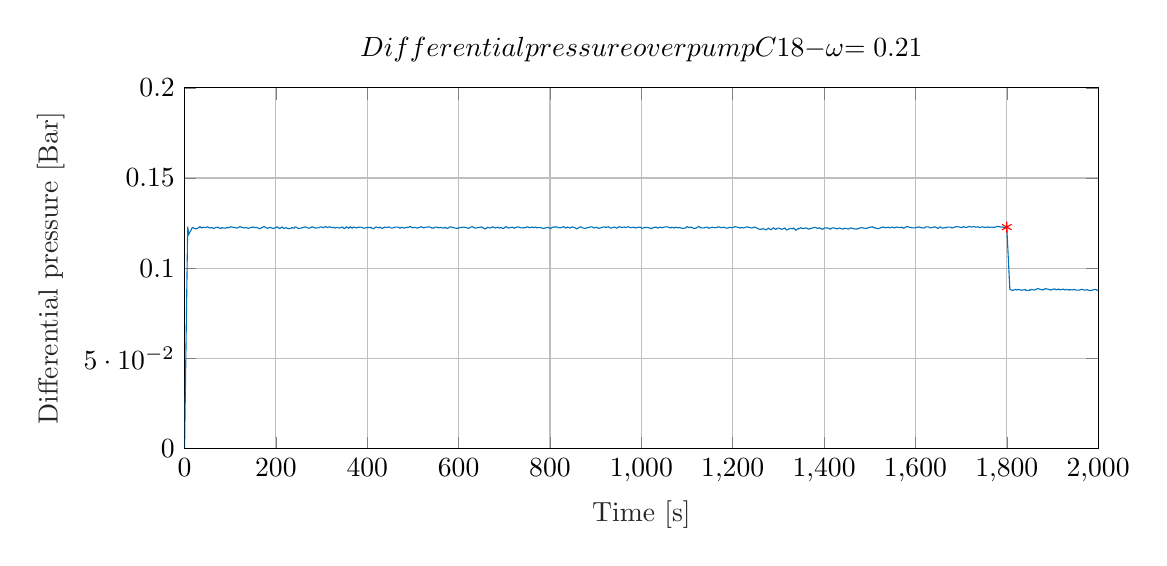
\begin{tikzpicture}

\begin{axis}[%
width=4.568in,
height=1.803in,
at={(0.78in,0.521in)},
scale only axis,
xmin=0,
xmax=2000,
xlabel style={font=\color{white!15!black}},
xlabel={Time [s]},
ymin=0,
ymax=0.2,
ylabel style={font=\color{white!15!black}},
ylabel={Differential pressure [Bar]},
axis background/.style={fill=white},
title style={font=\bfseries},
title={$\text{Differential pressure over pump C18 - }\omega\text{ = 0.21}$},
xmajorgrids,
ymajorgrids
]
\addplot [color=mycolor1, forget plot]
  table[row sep=crcr]{%
0	0\\
6.84999999999991	0.123002199413349\\
9.09999999999991	0.11876832844564\\
16.9499999999998	0.122470674486976\\
18.5	0.122421798631422\\
23.1500000000001	0.121847507331495\\
27.1500000000001	0.121920821114145\\
33.75	0.122989980449802\\
37.1999999999998	0.122336265884769\\
41.8499999999999	0.122745601172937\\
45.5500000000002	0.122476783968523\\
50.6999999999998	0.122934995112246\\
55.3499999999999	0.122214076246109\\
59.0999999999999	0.122580645161179\\
63.8000000000002	0.121981915933702\\
68.1999999999998	0.122598973607182\\
74.1500000000001	0.122702834799838\\
76.1500000000001	0.122189638318559\\
79.75	0.122018572825255\\
81.1500000000001	0.122489002932525\\
89.75	0.122152981427007\\
93.0500000000002	0.122660068426285\\
96.25	0.122403470185873\\
101.25	0.122934995112246\\
114.95	0.122256842619663\\
121.8	0.123044965786903\\
122.2	0.122886119257146\\
130.6	0.122293499511215\\
134.75	0.122495112414526\\
139.8	0.122116324535909\\
150.2	0.122867790811597\\
152.45	0.122476783968978\\
157.45	0.122635630498735\\
165	0.121878054741046\\
165.95	0.122055229716352\\
173.3	0.123032746822901\\
175.25	0.122947214076248\\
181.1	0.122055229716352\\
186.1	0.12258675464318\\
194.25	0.122024682306801\\
200.75	0.122617302052731\\
202.45	0.122892228739147\\
208.4	0.121963587487699\\
213.45	0.122843352883592\\
217.4	0.12199413489725\\
222.45	0.122489002932525\\
225.45	0.122030791788802\\
232.25	0.122006353861252\\
235.45	0.12256231671563\\
240.15	0.122189638318559\\
242	0.122843352883592\\
245.2	0.12273338220939\\
248.4	0.1219208211146\\
255.05	0.122226295210112\\
260.25	0.122653958944284\\
264.85	0.122837243401591\\
269.85	0.122342375366316\\
273.45	0.122146871945006\\
279.3	0.122947214076248\\
286.6	0.122262952101664\\
293.1	0.122397360703872\\
295.7	0.122733382208935\\
299.4	0.122898338220693\\
303.55	0.122452346040973\\
308.6	0.123051075268904\\
312.2	0.12258675464318\\
317.8	0.122934995112246\\
322.7	0.122470674486522\\
325.5	0.122672287389832\\
329.4	0.122299608993217\\
333.45	0.122641739980281\\
339.1	0.122220185728111\\
345.3	0.122843352883592\\
349.05	0.122055229716352\\
350.25	0.12199413489725\\
354.1	0.122947214076248\\
359.1	0.122116324535455\\
362.6	0.122910557184696\\
366.8	0.122152981427007\\
369.75	0.122837243401591\\
376.35	0.122299608993217\\
379.35	0.122660068426285\\
385.7	0.122770039100487\\
391.05	0.122293499511215\\
393.4	0.122214076246109\\
400.95	0.122537878787625\\
408.55	0.12258675464318\\
410.2	0.122146871945006\\
413.45	0.121914711632144\\
419.25	0.122825024438043\\
425.95	0.122360703812319\\
427.75	0.122776148582489\\
432.6	0.122012463342799\\
438.7	0.122837243401591\\
441.6	0.122501221896073\\
447.35	0.122861681329141\\
452.4	0.122226295210112\\
454.9	0.122226295210112\\
461.05	0.122733382208935\\
468.8	0.122739491690936\\
470.8	0.122281280547213\\
471.9	0.122159090909008\\
474.8	0.122696725317383\\
480.6	0.122244623655661\\
487.1	0.122708944281385\\
488.8	0.122495112414526\\
493.85	0.123124389051554\\
498.85	0.12236681329432\\
503.8	0.122690615835836\\
509.15	0.122220185728111\\
518.55	0.122934995112246\\
523.7	0.122336265884769\\
528.1	0.12275782013694\\
536.5	0.122904447702695\\
541.15	0.122275171065212\\
545.2	0.122244623655661\\
548.2	0.122684506353835\\
552.05	0.122800586510039\\
555.6	0.122360703812319\\
561.25	0.122598973606728\\
566.65	0.122195747800561\\
571.15	0.122690615835836\\
572.6	0.122195747800561\\
576.3	0.122152981427007\\
580.75	0.122928885630245\\
587.6	0.122629521016734\\
592.55	0.122220185728111\\
598.55	0.122079667643902\\
601.95	0.122543988269626\\
604.25	0.122464565004975\\
610.95	0.12280669599204\\
621.65	0.122128543499457\\
627.65	0.122880009775145\\
630.3	0.122983870967801\\
636.1	0.122201857282562\\
650.75	0.122861681329141\\
654.6	0.122171309873011\\
658.7	0.121755865102386\\
663.35	0.122660068426285\\
669.15	0.122250733137662\\
674.4	0.122934995112246\\
680.2	0.122305718474763\\
686	0.122739491690936\\
689.15	0.122238514174114\\
693.05	0.122550097751628\\
696.4	0.122012463342799\\
698.25	0.122061339198353\\
703.65	0.123008308895351\\
708.95	0.122244623655661\\
717.9	0.122745601172937\\
721.4	0.122183528836558\\
728.45	0.122873900293143\\
734.1	0.122653958944284\\
736.5	0.122348484848317\\
747.7	0.122482893450524\\
748.75	0.122861681329141\\
751.1	0.122861681329141\\
755.5	0.122372922775867\\
760.15	0.122855571847595\\
763.95	0.122458455522974\\
768.7	0.122855571847595\\
771.25	0.122385141739869\\
777.7	0.122598973606728\\
786.05	0.1220185728248\\
793.8	0.122653958944284\\
796	0.122666177907831\\
800.85	0.122000244379251\\
803.6	0.122403470185418\\
807.5	0.12280669599204\\
814.95	0.122843352883592\\
820.4	0.12239125122187\\
822	0.122385141739869\\
830.3	0.122989980449347\\
834.8	0.122256842619663\\
838.85	0.12280669599204\\
843.8	0.122256842619663\\
848.65	0.122880009775145\\
854.1	0.122495112414526\\
858.85	0.12179863147594\\
863.9	0.12263563049828\\
867.2	0.122916666666697\\
872.6	0.122238514174114\\
876.1	0.122036901270803\\
881.5	0.12239125122187\\
888.35	0.122855571847595\\
892.1	0.122886119257146\\
896.6	0.122275171065212\\
901.45	0.122684506353835\\
906.15	0.122146871945006\\
907.7	0.122159090909008\\
916.35	0.122794477028037\\
920.15	0.122904447702695\\
922.35	0.12256231671563\\
927.65	0.122983870967801\\
932.65	0.122207966764108\\
933.9	0.122250733137662\\
940.85	0.122837243401591\\
945.85	0.122189638318559\\
951.35	0.123002199413349\\
956.3	0.12258675464318\\
963.05	0.12283113391959\\
964.95	0.122507331378074\\
971.1	0.122953323558249\\
976.9	0.122452346040973\\
984.05	0.122727272727388\\
985.2	0.122452346040973\\
989.05	0.122330156402768\\
990.5	0.122556207233629\\
997.35	0.122763929618486\\
1000.9	0.122128543499457\\
1004.3	0.122256842619663\\
1006.5	0.122629521016734\\
1015.6	0.122501221896073\\
1021.15	0.121908602150597\\
1028.3	0.122666177907831\\
1032.75	0.122690615835836\\
1036.05	0.122201857282562\\
1041.05	0.122794477028037\\
1043.8	0.122427908113423\\
1053.7	0.122916666666697\\
1057.4	0.122904447702695\\
1064.1	0.122305718474763\\
1066.95	0.122751710654939\\
1071.95	0.122244623655661\\
1074.4	0.122715053763386\\
1080.45	0.12236681329432\\
1082.45	0.122568426197176\\
1089.65	0.122049120234351\\
1097.3	0.122317937438766\\
1099.65	0.122965542521797\\
1100.55	0.123008308895351\\
1104.15	0.122507331378074\\
1108.8	0.122812805474041\\
1114.35	0.122097996089906\\
1119.05	0.122122434017456\\
1125.05	0.123099951124004\\
1126.25	0.123075513196454\\
1129.95	0.122421798631422\\
1137.1	0.122311827956764\\
1142.4	0.12275782013694\\
1144.7	0.122788367546491\\
1147.4	0.122152981427007\\
1155.8	0.122763929618486\\
1157.25	0.122470674486522\\
1165.2	0.122476783968523\\
1166.7	0.122837243401591\\
1170	0.122910557184696\\
1174.4	0.122434017595424\\
1180.95	0.12275782013694\\
1184.9	0.122269061583665\\
1189.65	0.122244623655661\\
1193.1	0.122715053763386\\
1197.65	0.122409579667419\\
1205.8	0.123002199413349\\
1217.15	0.122305718474763\\
1218.1	0.122623411534732\\
1223.05	0.122317937438766\\
1231.35	0.122904447702695\\
1242.7	0.122214076246109\\
1246	0.12280669599204\\
1249.65	0.122678396871834\\
1256.65	0.121743646138839\\
1262.1	0.121474828934424\\
1265.75	0.121963587487699\\
1272.8	0.121279325513115\\
1278.1	0.122165200391009\\
1282.75	0.121383186705771\\
1283.8	0.121352639296219\\
1289.4	0.122385141739869\\
1294.3	0.121450391006874\\
1297.85	0.122201857282562\\
1301.7	0.122201857282562\\
1307.55	0.121523704789524\\
1313.9	0.122281280547213\\
1317.55	0.121315982404667\\
1318.5	0.121199902248009\\
1326.45	0.122091886607905\\
1331	0.12179863147594\\
1333.25	0.122262952101664\\
1338.2	0.121065493646256\\
1343.05	0.12199413489725\\
1344.1	0.121780303030391\\
1349.25	0.122427908113423\\
1352.85	0.121920821114145\\
1360.55	0.122372922775867\\
1365.95	0.121639784946183\\
1378.6	0.122598973606728\\
1380.65	0.122660068426285\\
1386.15	0.122036901270803\\
1389.6	0.122385141739869\\
1394.2	0.121737536656838\\
1397.85	0.121725317692835\\
1400.8	0.122342375366316\\
1410.5	0.122226295210112\\
1412.25	0.121731427174836\\
1415.15	0.12177419354839\\
1417.8	0.122372922775867\\
1424.3	0.122214076246109\\
1427.5	0.121768084066389\\
1434.1	0.122293499511215\\
1439.45	0.121743646138839\\
1442.1	0.121725317692835\\
1444.45	0.122152981427007\\
1454.05	0.121725317692835\\
1457.95	0.122342375366316\\
1465.8	0.121792521993939\\
1471.5	0.121615347018633\\
1473.15	0.122049120234351\\
1475.35	0.121896383186595\\
1480.65	0.122519550342076\\
1492.45	0.122012463342799\\
1498.25	0.122543988269626\\
1505.4	0.122947214076248\\
1509.9	0.122330156402768\\
1511	0.122427908113423\\
1516.25	0.12194525904215\\
1519.55	0.122036901270803\\
1529.4	0.122861681329141\\
1534.4	0.122385141739869\\
1541.05	0.122751710654939\\
1542.8	0.12236681329432\\
1545.35	0.122372922775867\\
1548.75	0.122855571847595\\
1553.8	0.12236681329432\\
1559.5	0.122800586510039\\
1568.75	0.122427908113423\\
1569.65	0.122745601172937\\
1574.65	0.122171309873011\\
1579.75	0.122928885630245\\
1583.3	0.123032746822901\\
1588.35	0.122550097751628\\
1589.85	0.122647849462282\\
1593.15	0.122379032257868\\
1599	0.122379032257868\\
1608.05	0.122880009775145\\
1612.2	0.122458455522974\\
1618.85	0.122262952101664\\
1622.8	0.122880009775145\\
1629.3	0.122867790811142\\
1631.05	0.122360703812319\\
1633.55	0.122317937438766\\
1640	0.122818914956042\\
1643.8	0.122855571847595\\
1648.8	0.122049120234351\\
1650	0.122183528836558\\
1654.25	0.122892228738692\\
1659.25	0.122195747800561\\
1666.95	0.122537878787625\\
1667.4	0.122427908113423\\
1670.3	0.122788367546491\\
1676.85	0.122776148582489\\
1679.85	0.122275171065212\\
1684.45	0.12261119257073\\
1688.85	0.123081622678455\\
1697.3	0.122788367546491\\
1700.25	0.122501221896073\\
1701.9	0.122531769306079\\
1704.45	0.122989980449347\\
1711.15	0.122574535679178\\
1717.75	0.123142717497558\\
1722.65	0.12280669599204\\
1728.65	0.123075513196454\\
1732.55	0.122733382208935\\
1736.85	0.122947214076248\\
1740.55	0.122543988269626\\
1745.55	0.122910557184696\\
1753.6	0.122550097751628\\
1758.05	0.122892228738692\\
1762.5	0.122592864125181\\
1767.05	0.122800586510039\\
1771.75	0.12256231671563\\
1779.15	0.123118279570008\\
1783.15	0.123057184750451\\
1788.1	0.122733382208935\\
1789.55	0.122916666666697\\
1797.8	0.122452346040973\\
1799.95	0.122794477028037\\
1806.65	0.0883797653959846\\
1811.75	0.0876405180838447\\
1819.75	0.0882453567937773\\
1821.75	0.0879337732158092\\
1826.75	0.0882086999022249\\
1831.3	0.0877504887585019\\
1840.25	0.0881720430106725\\
1841.45	0.0877321603129531\\
1849	0.087628299120297\\
1850.15	0.0879704301073616\\
1851.2	0.0878054740956031\\
1853.95	0.0882148093842261\\
1860.75	0.0878421309871555\\
1866	0.0885141739981918\\
1868.75	0.0886546920819455\\
1875.05	0.08808651026402\\
1880.4	0.0880254154449176\\
1883.85	0.0885997067448443\\
1885.35	0.0885813782988407\\
1893.95	0.0881353861191201\\
1896	0.0878238025416067\\
1904.05	0.0885508308892895\\
1908.15	0.0880131964809152\\
1913.85	0.0883980938415334\\
1915.7	0.087982649071364\\
1924.35	0.0883736559139834\\
1927.3	0.0879337732158092\\
1931.2	0.088257575757325\\
1936.4	0.0878115835776043\\
1937.8	0.0881720430106725\\
1943.1	0.0878971163242568\\
1946.8	0.0882270283477737\\
1951.75	0.0878054740956031\\
1959.35	0.0878848973607091\\
1963.85	0.0882881231668762\\
1970.95	0.0878054740956031\\
1975.9	0.0880681818180165\\
1981.4	0.087524437927641\\
1994.4	0.0882453567937773\\
1997.85	0.0877260508309519\\
2000.7	0.0875977517107458\\
2013.3	0.0881414956011213\\
2018.8	0.0874938905180898\\
2024.25	0.0879398826978104\\
2025.3	0.0877504887585019\\
2037.3	0.088031524926464\\
2040.85	0.0877016129029471\\
2052.85	0.0882636852393262\\
2057.95	0.0878115835776043\\
2063.3	0.0877871456500543\\
2068.3	0.0882453567937773\\
2070.35	0.0882392473117761\\
2076.1	0.0879215542522616\\
2077.85	0.0880376344084652\\
2083.75	0.0877321603129531\\
2086.2	0.0879521016618128\\
2096.3	0.0883003421308786\\
2105.3	0.0877810361680531\\
2111.35	0.0881353861191201\\
2117.3	0.0877749266860519\\
2120.3	0.0882636852393262\\
2123.75	0.0887035679375003\\
2128.3	0.0879398826978104\\
2136.25	0.0889846041054625\\
2139.5	0.0884775171066394\\
2144.4	0.0893450635385307\\
2152.05	0.0884714076246382\\
2155.7	0.089173998044771\\
2159.55	0.0893939393940855\\
2163.6	0.089070136852115\\
2166.75	0.0891373411532186\\
2172.05	0.0899437927664621\\
2177.1	0.0890579178885673\\
2182.05	0.0897605083087001\\
2185.95	0.0890151515150137\\
2195.85	0.0898216031278025\\
2197.9	0.0895100195502891\\
2202.9	0.0899254643204586\\
2208.3	0.0893389540569842\\
2210.45	0.0898338220922597\\
2219.65	0.0887952101666087\\
2225.7	0.0900354349955705\\
2234.55	0.089338954057439\\
2241.25	0.0900598729235753\\
2243.25	0.0896444281529511\\
2248.85	0.0899743401764681\\
2252.8	0.0899499022489181\\
2257.95	0.0891617790816781\\
2261.6	0.0894978005871963\\
2263.25	0.0898521505382632\\
2271.3	0.0893511730209866\\
2276.35	0.0898765884658133\\
2283	0.0900354349955705\\
2286.65	0.0895711143698463\\
2289.2	0.0897849462371596\\
2295.7	0.0891923264912293\\
2304.2	0.0900415444775717\\
2311.45	0.0892473118283306\\
2315.35	0.0892534213103318\\
2320.35	0.089766617791156\\
2325.2	0.0893084066478878\\
2330.55	0.090096529814673\\
2339.05	0.0895100195507439\\
2340.55	0.0892106549372329\\
2344	0.0897788367551584\\
2349	0.0889601661783672\\
2356.25	0.0899682306944669\\
2357.2	0.0898888074298156\\
2361.2	0.0894000488765414\\
2365.2	0.0894733626591915\\
2367	0.0899560117304645\\
2374.45	0.0898582600202644\\
2379.1	0.0890701368530245\\
2383.9	0.0899010263933633\\
2391.1	0.0891067937445769\\
2393.3	0.0891129032265781\\
2396.95	0.0896871945265048\\
2402.15	0.0895772238518475\\
2406.9	0.088954056696366\\
2408.9	0.0891617790816781\\
2415.5	0.0899926686220169\\
2417.6	0.089821603128712\\
2423.55	0.0892106549367782\\
2426.3	0.089363391984989\\
2428.6	0.089717741936056\\
2438.25	0.0897727272731572\\
2441	0.0890212609979244\\
2443.75	0.0891251221901257\\
2451.05	0.0899254643213681\\
2457.8	0.0898277126107132\\
2460.2	0.0892900782018842\\
2461.2	0.0894611436956438\\
2466.15	0.0887768817210599\\
2473.9	0.0888929618772636\\
2478.7	0.0895588954062987\\
2481.8	0.0901148582606766\\
2487.75	0.0890762463350256\\
2493.5	0.0900476539595729\\
2501.6	0.0897482893456072\\
2504.15	0.0892473118283306\\
2508.45	0.0899010263933633\\
2512.55	0.0892656402743341\\
2516.15	0.0896810850445036\\
2518.7	0.0891862170092281\\
2523.5	0.0892167644187793\\
2528.6	0.0900598729231206\\
2532.35	0.0899926686220169\\
2534.7	0.0896138807433999\\
2539.75	0.08963831867095\\
2541.6	0.0891190127081245\\
2549.7	0.0892228739007805\\
2555.9	0.0899193548393669\\
2559.25	0.0897605083091548\\
2565.3	0.0887096774199563\\
2567.55	0.0894978005871963\\
2577.7	0.0892412023463294\\
2582.75	0.0887891006850623\\
2587.8	0.0894794721411927\\
2592.15	0.0887707722390587\\
2597	0.0894794721411927\\
2602.45	0.0885080645166454\\
2608	0.0894978005871963\\
2610.7	0.0894489247316415\\
2616.7	0.0888379765401623\\
2618.3	0.0891801075272269\\
2623.8	0.0883308895408845\\
2627.2	0.0887157869019575\\
2634.9	0.0897055229720536\\
2637.7	0.0897910557191608\\
2644.7	0.0886119257093014\\
2649.75	0.0894794721411927\\
2653.5	0.0895222385147463\\
2659.6	0.0889907135879184\\
2662.7	0.0890762463350256\\
2665.85	0.0884408602155418\\
2672.45	0.0886485826008538\\
2679.4	0.0891617790816781\\
2683.25	0.0896016617793975\\
2687.6	0.0889968230699196\\
2692.85	0.0899437927669169\\
2703.05	0.0887646627570575\\
2705.2	0.0891984359732305\\
2708.05	0.0892473118283306\\
2713.35	0.0888379765401623\\
2716.25	0.0887891006846075\\
2721.95	0.0895833333338487\\
2724.8	0.0895527859242975\\
2729.8	0.0883858748784405\\
2731.8	0.0886302541548503\\
2736.2	0.0896444281529511\\
2743.6	0.0898093841647096\\
2749.3	0.0883797653964393\\
2758	0.0892900782018842\\
2766.05	0.0887035679379551\\
2772.2	0.0885202834806478\\
2775	0.0890518084074756\\
2777.55	0.089338954057439\\
2782.1	0.0885874877817514\\
2784.25	0.0890212609974697\\
2787.55	0.0894794721411927\\
2795.8	0.0888929618772636\\
2802.3	0.0896994134905071\\
2807.35	0.0890701368530245\\
2813.7	0.089363391984989\\
2815.6	0.0888563049857112\\
2820.65	0.089259530792333\\
2827.75	0.0886730205284039\\
2829.4	0.0892900782018842\\
2835.35	0.0884591886615453\\
2840.35	0.0891923264912293\\
2845.4	0.0886485826008538\\
2850.55	0.0894794721411927\\
2858.8	0.0890518084070209\\
2862	0.0894305962860926\\
2864.2	0.0893939393945402\\
2871.1	0.0884836265886406\\
2875.95	0.0891801075276817\\
2879.85	0.0884897360710966\\
2881.2	0.088495845552643\\
2887.9	0.0891251221901257\\
2891.8	0.0888563049857112\\
2896.8	0.0894794721411927\\
2898.8	0.0894244868040914\\
2905.95	0.0889968230699196\\
2912.2	0.0888990713592648\\
2915.1	0.089467253177645\\
2920	0.0889418377328184\\
2927.25	0.0891495601176757\\
2932.2	0.0898277126107132\\
2936.2	0.0891923264912293\\
2941.25	0.0897543988276084\\
2946.4	0.0887280058655051\\
2960.75	0.089742179863606\\
2967.8	0.0886302541548503\\
2973.65	0.0896444281529511\\
2978	0.0897360703820596\\
2984.45	0.0886730205284039\\
2986.3	0.0887768817210599\\
2991.35	0.0895833333338487\\
2993.6	0.0891617790816781\\
3002.25	0.0897543988276084\\
3003.25	0.0899376832849157\\
3008.2	0.0889235092868148\\
3011.4	0.089283968719883\\
3018.6	0.0888929618772636\\
3020.8	0.088905180841266\\
3022.55	0.0893695014669902\\
3028.85	0.0891984359732305\\
3032.65	0.0887891006846075\\
3037.25	0.088905180841266\\
3047.6	0.0897055229720536\\
3054.5	0.0891006842625757\\
3058.2	0.0895894428158499\\
3063.05	0.0891801075272269\\
3066.2	0.0891984359732305\\
3072.15	0.0897116324540548\\
3072.9	0.0900048875860193\\
3077.5	0.0889723851423696\\
3084.85	0.0898582600202644\\
3089.6	0.0888929618772636\\
3095.35	0.0896444281529511\\
3100.45	0.0893817204305378\\
3104.4	0.0898399315742608\\
3111.2	0.0897849462371596\\
3116.15	0.0892228739007805\\
3124.5	0.0898521505382632\\
3125.05	0.0900904203326718\\
3130.05	0.0888196480941588\\
3134.9	0.0899315738033692\\
3139.55	0.0888563049857112\\
3142.4	0.0892961876838854\\
3147.3	0.0898765884658133\\
3154.15	0.0899560117304645\\
3157.5	0.0891617790816781\\
3164.65	0.089009042033922\\
3167.3	0.089742179863606\\
3168.4	0.0896933040085059\\
3173.5	0.0887891006846075\\
3177.65	0.0891617790816781\\
3184.25	0.0894367057676391\\
3185.6	0.089338954057439\\
3194.35	0.0902675953084326\\
3200.8	0.0892534213103318\\
3207	0.0894550342136426\\
3209.8	0.0897727272731572\\
3214.3	0.0891984359732305\\
3218.7	0.0897727272731572\\
3221.15	0.0896322091889488\\
3224.1	0.0891984359732305\\
3229.65	0.0893328445754378\\
3234	0.0900537634411194\\
3242.5	0.0899560117309193\\
3246.7	0.0890762463350256\\
3248.15	0.0890640273710233\\
3257.35	0.0899010263933633\\
3262.85	0.0894183773220902\\
3267.25	0.0894305962860926\\
3273.3	0.0900782013691241\\
3278.45	0.0894244868040914\\
3287.6	0.0900537634415741\\
3291.1	0.0895527859242975\\
3296.1	0.090151515152229\\
3299.15	0.0901087487786754\\
3307.8	0.0893572825029878\\
3313.05	0.090072091887123\\
3319.2	0.0893328445754378\\
3324.2	0.0901637341157766\\
3327.6	0.090096529814673\\
3330.7	0.0896810850445036\\
3338.15	0.0893328445754378\\
3341.9	0.090224828934879\\
3347.3	0.0901820625617802\\
3349.95	0.0897116324540548\\
3352.65	0.0895650048882999\\
3356.2	0.0899499022489181\\
3366.5	0.0895650048882999\\
3367.55	0.0899193548393669\\
3370.15	0.0901209677426777\\
3375.4	0.0895405669602951\\
3379.45	0.0899926686220169\\
3385.1	0.0895650048882999\\
3389.8	0.0902614858264315\\
3394.85	0.0895100195507439\\
3395.1	0.0896199902254011\\
3396.7	0.0901454056702278\\
3404.95	0.090120967742223\\
3409	0.0897727272731572\\
3414.05	0.0900354349955705\\
3420.9	0.0891006842625757\\
3421.5	0.0891739980452257\\
3429.55	0.0904569892477411\\
3430.25	0.0904569892477411\\
3436.9	0.0896871945265048\\
3440.85	0.0900598729231206\\
3445	0.0896994134900524\\
3451.4	0.0892534213103318\\
3455.6	0.0899437927669169\\
3459.6	0.0895039100691974\\
3464.9	0.0904753176937447\\
3471.15	0.0894305962860926\\
3477.9	0.0900598729235753\\
3481.2	0.0897238514180572\\
3487.1	0.0902126099713314\\
3492.05	0.0895100195507439\\
3506.3	0.0902981427179839\\
3509.6	0.0902431573804279\\
3515.4	0.0897482893456072\\
3520.45	0.0899804496584693\\
3523.5	0.0895772238518475\\
3526.05	0.0896688660805012\\
3529.2	0.0900782013691241\\
3534.75	0.0897299608996036\\
3543.95	0.090096529814673\\
3549.4	0.0896810850445036\\
3556.15	0.0900476539595729\\
3559.25	0.0897360703820596\\
3564.05	0.0901454056702278\\
3567.95	0.0896322091889488\\
3573.05	0.0903103616819863\\
3578.1	0.0894733626591915\\
3578.35	0.0895405669602951\\
3582.65	0.0901148582606766\\
3587.8	0.089821603128712\\
3593.65	0.0901270772242242\\
3600.55	0.089821603128712\\
3604.55	0.215591397849948\\
3609.75	0.280565738025871\\
3615.5	0.280076979472597\\
3619.65	0.280620723362972\\
3630.2	0.279423264907564\\
3634.1	0.279184995112701\\
3642.2	0.280046432063045\\
3647.2	0.279343841642458\\
3652.2	0.280138074291699\\
3654.65	0.279545454545769\\
3659.5	0.279973118279941\\
3664.15	0.27960043988287\\
3665.9	0.279728739003076\\
3673.45	0.279294965787358\\
3680.9	0.279349951124459\\
3682.85	0.279905913978837\\
3686.6	0.280333577713009\\
3691.65	0.279557673509771\\
3695.05	0.279618768328874\\
3698.3	0.280113636364149\\
3705.4	0.280095307918145\\
3708.15	0.279594330401324\\
3709.55	0.27974706744908\\
3715.45	0.279032258064944\\
3720.55	0.280107526882148\\
3725.2	0.27952712610022\\
3726.75	0.279912023460838\\
3735.75	0.279233870967801\\
3743.9	0.278183040078602\\
3747.5	0.277877565982635\\
3752.6	0.278574046921221\\
3753.5	0.278488514174114\\
3761.65	0.266666666666879\\
3763.7	0.262573313783378\\
3770.35	0.264791055718888\\
3779.1	0.267228739003258\\
3787.8	0.270002443793146\\
};
\addplot [color=red, draw=none, mark=asterisk, mark options={solid, red}, forget plot]
  table[row sep=crcr]{%
1800	0.122794477028265\\
};
\addplot [color=red, draw=none, mark=asterisk, mark options={solid, red}, forget plot]
  table[row sep=crcr]{%
3600	0.0899865591404705\\
};
\end{axis}
\end{tikzpicture}%
\caption{Small signal measurements for pump C18.}
\label{fig:small_sig_diff_press_C18}
\end{figure}

\begin{figure}[H]
% This file was created by matlab2tikz.
%
%The latest updates can be retrieved from
%  http://www.mathworks.com/matlabcentral/fileexchange/22022-matlab2tikz-matlab2tikz
%where you can also make suggestions and rate matlab2tikz.
%
\definecolor{mycolor1}{rgb}{0.00000,0.44700,0.74100}%
%
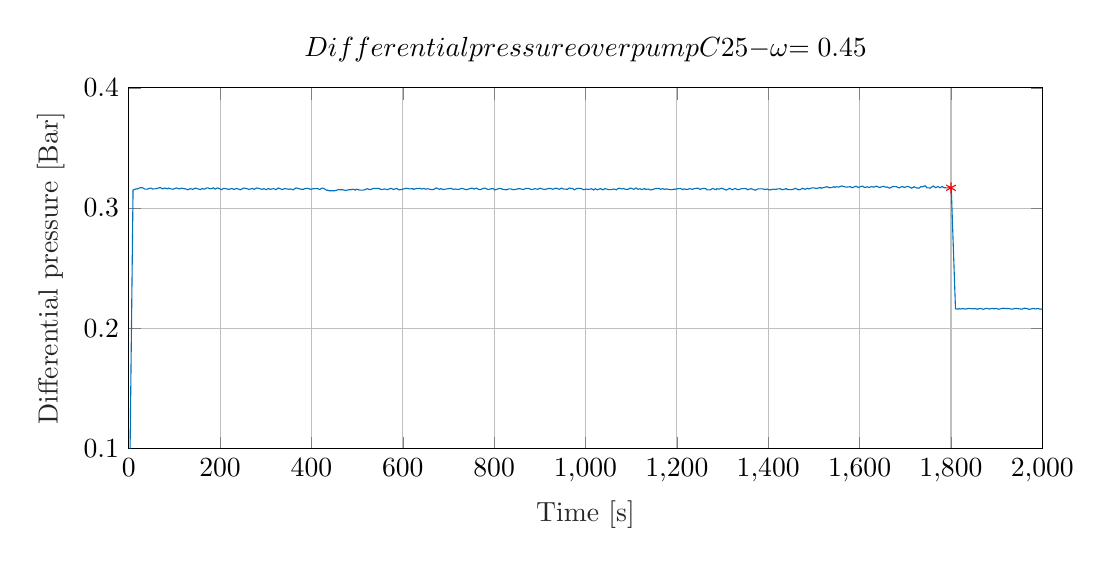
\begin{tikzpicture}

\begin{axis}[%
width=4.568in,
height=1.803in,
at={(0.766in,0.486in)},
scale only axis,
xmin=0,
xmax=2000,
xlabel style={font=\color{white!15!black}},
xlabel={Time [s]},
ymin=0.1,
ymax=0.4,
ylabel style={font=\color{white!15!black}},
ylabel={Differential pressure [Bar]},
axis background/.style={fill=white},
title style={font=\bfseries},
title={$\text{Differential pressure over pump C25 - }\omega\text{ = 0.45}$},
xmajorgrids,
ymajorgrids
]
\addplot [color=mycolor1, forget plot]
  table[row sep=crcr]{%
0	0\\
9.5	0.314980449657924\\
16.75	0.316092375366679\\
19	0.315854105571816\\
23.5	0.316776637340809\\
29.75	0.317002688171669\\
35.0500000000002	0.315793010752714\\
40.5500000000002	0.31570136852406\\
46.75	0.31661168132905\\
49.25	0.316630009775508\\
51.75	0.31589687194537\\
57.6000000000004	0.315951857282926\\
69.1999999999998	0.31708211143723\\
74.9499999999998	0.315939638318923\\
79.0500000000002	0.316746089931257\\
83.8999999999996	0.31599462365557\\
87.8500000000004	0.316623900293052\\
90.4499999999998	0.316110703812228\\
96.8000000000002	0.315658602150506\\
104.35	0.316764418377716\\
110.7	0.315921309873374\\
115.6	0.31661168132905\\
123	0.315927419354921\\
123.65	0.316202346040882\\
129.05	0.315169843597687\\
135.2	0.316220674486431\\
140.4	0.31555474095785\\
142.4	0.316043499511579\\
145.95	0.316575024437952\\
157.05	0.315347018572538\\
160.65	0.316263440859984\\
165.35	0.315676930596055\\
170.45	0.316642228738601\\
172.65	0.316837732159911\\
178.75	0.31594574780047\\
185.5	0.316825513196818\\
188.75	0.315841886607814\\
189.7	0.315817448680718\\
194.7	0.316788856304811\\
203.2	0.315340909090992\\
207.55	0.316385630499099\\
209.85	0.316355083089547\\
217.1	0.315695259042513\\
220.55	0.315689149560058\\
225.65	0.316275659823987\\
230.7	0.315487536657201\\
235.5	0.316281769306443\\
236.9	0.316214565004884\\
244.7	0.315243157380792\\
246.6	0.315664711632962\\
251.6	0.316617790811506\\
257.85	0.31631842619754\\
262.85	0.315524193548299\\
271.15	0.316300097751991\\
275.05	0.315579178885855\\
280.05	0.316752199413713\\
286.9	0.316135141740233\\
291.95	0.31550586510275\\
295.8	0.316177908113787\\
300.95	0.315310361681441\\
305.95	0.316293988270445\\
309.35	0.315560850440306\\
317.25	0.31622067448734\\
322.2	0.315304252199894\\
327.65	0.316691104594611\\
336.25	0.315353128054994\\
341.45	0.316245112414435\\
350.65	0.315634164223411\\
353.8	0.315957966764472\\
360.15	0.315224828934333\\
366.3	0.316770527859262\\
377.8	0.315634164223411\\
383.3	0.315646383186504\\
385.6	0.31626955034244\\
392.7	0.316422287390196\\
397.6	0.315597507331404\\
398.45	0.315597507331404\\
403.45	0.316092375366679\\
413.85	0.316263440859984\\
416.75	0.31560361681295\\
418.7	0.315493646138748\\
422.95	0.316630009774599\\
426.45	0.316434506353289\\
433.6	0.314760508308609\\
435.9	0.314815493646165\\
437.75	0.314442815249095\\
450.8	0.314406158357087\\
454.85	0.314821603127712\\
459.35	0.315316471162987\\
468.2	0.315218719451877\\
474.7	0.314662756598409\\
482.8	0.315340909090992\\
483.3	0.31513318670568\\
491.2	0.315676930596055\\
496.35	0.314992668621016\\
497.9	0.315664711632053\\
502.25	0.315408113391641\\
504.8	0.314943792765916\\
513.85	0.314919354838821\\
522.35	0.316104594329772\\
527.6	0.315328690126989\\
530.7	0.31560361681295\\
535.75	0.31636730205264\\
548.1	0.316410068426194\\
549.65	0.315786901270258\\
550.55	0.315872434017365\\
553.2	0.315322580644533\\
560.2	0.315957966764472\\
566.5	0.315249266862338\\
568.6	0.315683040077602\\
574.15	0.316458944281294\\
579.25	0.315438660801192\\
586.2	0.316293988269535\\
587.55	0.316220674486431\\
591.15	0.315127077223224\\
597.35	0.315456989246741\\
607.75	0.316489491690845\\
614.35	0.315988514174023\\
622.25	0.316092375366679\\
623.6	0.315591397848948\\
625.900000000001	0.31575024437916\\
629.150000000001	0.316287878787989\\
638.05	0.316446725317292\\
641.3	0.315811339198262\\
646.35	0.316342864124636\\
650.25	0.315664711632053\\
654.35	0.316086265884223\\
662.5	0.315377565982089\\
667.95	0.315469208210743\\
672.8	0.316746089931257\\
680.75	0.31560361681295\\
683.7	0.316251221895982\\
688.5	0.315322580644533\\
692.1	0.315695259041604\\
705.75	0.316458944281294\\
710.05	0.315511974584297\\
710.95	0.315469208210743\\
715	0.315878543498911\\
721.400000000001	0.315426441837189\\
728.7	0.316410068426194\\
730.400000000001	0.316312316715084\\
738.95	0.315261485825431\\
740.5	0.315395894427638\\
748.6	0.316403958943738\\
751.150000000001	0.316544477028401\\
756.2	0.315811339198262\\
761.150000000001	0.316617790811506\\
767.05	0.315328690126989\\
770.900000000001	0.315353128054085\\
774.1	0.316147360703326\\
780.6	0.316593352883501\\
785.6	0.315579178884946\\
788.3	0.315530303029846\\
796.8	0.316306207233538\\
801.85	0.315096529813673\\
811.55	0.316403958943738\\
815.45	0.316165689149784\\
817.85	0.315670821114509\\
826.85	0.315175953079233\\
832.6	0.31602517106603\\
836.7	0.316012952102028\\
839.6	0.315420332356553\\
845.45	0.315383675464545\\
852.55	0.316116813294684\\
856.7	0.316086265885133\\
864.05	0.315322580645443\\
869.1	0.316397849463101\\
875.3	0.316379521016643\\
880.3	0.315591397849857\\
883.650000000001	0.315475317693199\\
889.3	0.316141251221779\\
895.5	0.315560850440306\\
899.8	0.316587243401955\\
905.1	0.315909090909372\\
912	0.315469208211653\\
917.75	0.316245112414435\\
923.85	0.316239002932889\\
928.25	0.315658602150506\\
928.7	0.315750244380069\\
936.45	0.316544477028401\\
942.35	0.315548631476304\\
947.7	0.316617790811506\\
951.650000000001	0.315817448680718\\
960.45	0.315621945259409\\
963.6	0.316630009775508\\
971.6	0.316306207233538\\
975.650000000001	0.315175953079233\\
976.05	0.315230938416789\\
981	0.316336754643999\\
989.75	0.316361192571094\\
995	0.31540811339255\\
996.6	0.315255376344794\\
1001.35	0.315854105571816\\
1005.45	0.315420332356553\\
1013.1	0.316067937439584\\
1018.2	0.315078201369033\\
1021.35	0.316092375366679\\
1026.2	0.315224828935243\\
1032.9	0.316239002932889\\
1037.9	0.315120967742587\\
1042.45	0.316184017595333\\
1050.7	0.31535923753745\\
1056.55	0.315292033235892\\
1061.35	0.31589687194537\\
1067.85	0.315224828934333\\
1070.25	0.316055718475582\\
1074.4	0.316544477028401\\
1079.75	0.315909090909372\\
1082.9	0.31631842619754\\
1087.9	0.315536412512301\\
1094.5	0.315713587488062\\
1096.85	0.316550586510857\\
1099.55	0.31646505376375\\
1105.8	0.315615835777862\\
1110.85	0.316727761485708\\
1114.95	0.315597507331404\\
1119.5	0.316061827957128\\
1123.45	0.315395894428548\\
1129.35	0.316251221896891\\
1130.9	0.315511974585206\\
1137.6	0.315841886608723\\
1141.3	0.315096529814582\\
1147.5	0.31540811339255\\
1152.05	0.316135141740233\\
1160.75	0.316403958944647\\
1164.05	0.315621945259409\\
1168.75	0.316147360704235\\
1173	0.315481427175655\\
1176.2	0.315976295210021\\
1184.25	0.315377565982999\\
1190	0.315304252199894\\
1193.65	0.315731915933611\\
1195.95	0.315560850440306\\
1201.05	0.316110703812228\\
1208.3	0.316257331378438\\
1213	0.315279814271889\\
1215.5	0.315945747801379\\
1222.4	0.315426441838099\\
1227.95	0.316208455523338\\
1233.8	0.315573069404309\\
1240.45	0.316373411535096\\
1246.2	0.31661168132996\\
1250.6	0.31550586510275\\
1251.2	0.315487536657201\\
1255.45	0.316306207233538\\
1262.75	0.31622067448734\\
1266.1	0.315102639296128\\
1273.05	0.315194281525692\\
1278.1	0.316306207233538\\
1286	0.315279814271889\\
1287.7	0.316159579668238\\
1292.7	0.315738025416067\\
1297.8	0.31656280547395\\
1307.7	0.315029325513933\\
1308.45	0.31498655914038\\
1315.7	0.316410068426194\\
1321.5	0.315237047898336\\
1327.85	0.316379521016643\\
1332.85	0.315279814271889\\
1336.35	0.31545698924765\\
1342.1	0.316159579668238\\
1351.2	0.316251221896891\\
1354.25	0.315292033235892\\
1362.55	0.316141251222689\\
1364.55	0.315835777126267\\
1372.1	0.314858260019719\\
1374.4	0.315310361681441\\
1376.75	0.315915200390918\\
1388.85	0.315982404692477\\
1393	0.315334799609445\\
1397.1	0.315866324535818\\
1402.95	0.315078201369033\\
1411.9	0.31579912023517\\
1415.05	0.315353128054994\\
1419.4	0.315884652982277\\
1426.65	0.316086265885133\\
1430.15	0.315261485826341\\
1431.15	0.315292033235892\\
1440.35	0.31622067448734\\
1441.55	0.315389784946092\\
1452.65	0.315316471163896\\
1458.4	0.316257331378438\\
1460.65	0.316263440860894\\
1466.2	0.315157624633684\\
1470.25	0.315444770283648\\
1475.15	0.316471163245296\\
1480.9	0.315579178885855\\
1486.15	0.316526148582852\\
1489.3	0.315872434018274\\
1494.9	0.316739980449711\\
1499.15	0.316862170087916\\
1505.15	0.316281769306443\\
1514.6	0.317173753665884\\
1515.7	0.316452834799748\\
1516.15	0.31651392961885\\
1528.55	0.317827468231371\\
1533.55	0.316898826979923\\
1538.85	0.31703323558213\\
1543.75	0.317864125122469\\
1545.5	0.317192082111433\\
1550.15	0.31779692082182\\
1554.9	0.317412023460747\\
1560.45	0.318407869012844\\
1571.1	0.317369257087194\\
1579.9	0.317851906158467\\
1582.2	0.317112658846781\\
1585.9	0.317185972629886\\
1592	0.318224584555537\\
1596.95	0.317137096774786\\
1606.1	0.318279569893093\\
1611.6	0.317002688172579\\
1616.65	0.317729716520262\\
1620.5	0.317100439882779\\
1625.9	0.317906891496023\\
1630.85	0.317363147605647\\
1636.9	0.31823680351954\\
1643.75	0.317106549364325\\
1652.35	0.31813905180843\\
1656.75	0.317369257087194\\
1660.25	0.31760141740051\\
1665.35	0.316568914956406\\
1673.3	0.317980205279127\\
1680.95	0.317754154448266\\
1686.5	0.316776637340809\\
1686.85	0.316849951123913\\
1693.5	0.318029081134227\\
1697.75	0.317185972629886\\
1705	0.318059628543779\\
1707.45	0.317839687194464\\
1714.15	0.316550586509948\\
1719.35	0.317729716520262\\
1724.35	0.316807184751269\\
1730	0.316532258065308\\
1733.75	0.317784701857818\\
1738.35	0.31774804496672\\
1743.6	0.318578934507059\\
1747.7	0.316794965787267\\
1754.9	0.316715542522616\\
1761.35	0.318340664712196\\
1766.7	0.316917155425472\\
1771.55	0.317998533724676\\
1776.1	0.316862170087916\\
1781.15	0.317967986315125\\
1781.5	0.317735826002718\\
1785.15	0.316917155425472\\
1794.2	0.316770527859262\\
1797.85	0.317405913979201\\
1800.65	0.316880498534374\\
1809.9	0.216122922776776\\
1816.05	0.216000733137662\\
1818.8	0.216306207234084\\
1820.5	0.216031280548123\\
1825.35	0.216342864126091\\
1830.6	0.216000733138571\\
1840.55	0.216495601172937\\
1847.15	0.216153470186327\\
1854.05	0.216342864125181\\
1857.7	0.215811339198808\\
1862.4	0.2165383675474\\
1871.35	0.215780791789257\\
1876.25	0.216520039100942\\
1879	0.216599462365593\\
1884	0.215909090909918\\
1889.95	0.216562805474496\\
1894.5	0.216177908114332\\
1899.25	0.216446725317837\\
1904.7	0.215847996090815\\
1914.9	0.216703323558249\\
1919.5	0.216318426198086\\
1923.7	0.216513929619396\\
1934.4	0.215860215053908\\
1938.55	0.216397849462737\\
1944.7	0.216440615836291\\
1955.3	0.215854105572362\\
1960.3	0.216672776149608\\
1966.2	0.216526148583398\\
1969.8	0.215854105572362\\
1972	0.215829667644357\\
1978.95	0.216367302053186\\
1982.6	0.216477272727388\\
1983.95	0.216061827957674\\
1990.4	0.216397849462737\\
1996.25	0.215835777126813\\
2000.15	0.216232893450979\\
2007.65	0.216617790812052\\
2015.35	0.216501710655393\\
2017.2	0.216104594331227\\
2020.35	0.215902981427462\\
2025.75	0.216440615836291\\
2030.3	0.21606793743922\\
2035.35	0.216758308895805\\
2039.65	0.215896871945915\\
2045.25	0.216593352884047\\
2047.45	0.216697214076703\\
2056.75	0.216049608993671\\
2060.35	0.216422287390742\\
2068.2	0.216208455523883\\
2072.55	0.216752199414259\\
2075.3	0.216477272728298\\
2077.55	0.21597018572902\\
2088.35	0.216318426198086\\
2094.7	0.216623900293598\\
2099.75	0.21569525904215\\
2104.8	0.216568914956042\\
2110.35	0.215933528837013\\
2118.1	0.21616568915033\\
2122.1	0.216593352884047\\
2126.2	0.216709433040705\\
2132.3	0.215738025415703\\
2141.25	0.216556695992949\\
2148.15	0.216275659824532\\
2149.7	0.216599462366503\\
2151.85	0.21641006842674\\
2155.5	0.215805229717262\\
2163.85	0.216526148583398\\
2166.8	0.215896871945006\\
2171.8	0.216184017595879\\
2174.1	0.215756353861252\\
2181.4	0.216012952101664\\
2186.35	0.216422287390742\\
2193.1	0.216092375367225\\
2196.15	0.216581133920045\\
2201.15	0.215988514173659\\
2205.35	0.216428396872288\\
2208.85	0.216452834800293\\
2215.35	0.216049608993671\\
2217.4	0.216147360703872\\
2221.35	0.216746089931803\\
2229.15	0.216739980450257\\
2234.2	0.216074046920767\\
2237.2	0.216416177908286\\
2242.2	0.216043499512125\\
2247.7	0.215866324536364\\
2252.2	0.216825513196454\\
2260.6	0.216599462365593\\
2262.8	0.216080156403223\\
2265.55	0.215976295210567\\
2275.25	0.216471163245842\\
2279.1	0.216000733138571\\
2287.35	0.216324535679632\\
2293.45	0.215713587488608\\
2298.05	0.21650782013694\\
2302.65	0.215793010753259\\
2308.95	0.216306207234084\\
2312.55	0.216074046921676\\
2317.05	0.2165872434025\\
2325.1	0.21641006842674\\
2329.6	0.215841886608359\\
2338.8	0.216550586510493\\
2340.95	0.216049608993671\\
2347.35	0.216623900293598\\
2351	0.216336754643635\\
2358.5	0.215982404693023\\
2363.6	0.216428396872288\\
2368.65	0.215994623656115\\
2371.15	0.215976295210567\\
2377.35	0.216678885631154\\
2383.65	0.216159579667874\\
2385.9	0.216568914956042\\
2388.15	0.216440615836291\\
2390.9	0.21611681329432\\
2399.8	0.215976295210567\\
2401.9	0.216269550342986\\
2407.2	0.215957966765018\\
2418.2	0.216721652003798\\
2421.45	0.216312316716539\\
2426.45	0.216636119257601\\
2434.95	0.215945747801015\\
2436.05	0.216037390029669\\
2443.4	0.216507820137849\\
2448.45	0.215994623656115\\
2455.15	0.216886608016466\\
2462.9	0.216000733138571\\
2470.9	0.216697214076703\\
2480.95	0.216159579667874\\
2481.9	0.216416177908286\\
2483.1	0.216239002933435\\
2488.15	0.216636119257601\\
2492.65	0.216575024438498\\
2504.5	0.215780791789257\\
2509.5	0.216684995112701\\
2512.3	0.216568914956042\\
2517.3	0.215939638319469\\
2520.75	0.215964076246564\\
2525.9	0.216581133920045\\
2534.7	0.216177908113423\\
2545.65	0.216025171065667\\
2548.75	0.216501710655393\\
2553.35	0.215872434017911\\
2556.5	0.216471163245842\\
2560.3	0.216135141740779\\
2563.65	0.216623900293598\\
2568.7	0.216208455523883\\
2573.7	0.216837732160457\\
2580.6	0.216611681329596\\
2585.6	0.216098484848771\\
2586.95	0.216379521017188\\
2590.2	0.216037390029669\\
2596.45	0.216281769306079\\
2605.1	0.215854105572362\\
2607	0.215988514174569\\
2614.1	0.216623900293598\\
2615.95	0.216636119257601\\
2620.95	0.216239002933435\\
2624.85	0.216318426198086\\
2628.35	0.216025171065667\\
2635.75	0.216043499511215\\
2641.2	0.216422287390742\\
2649.25	0.216055718475218\\
2654.3	0.216483382209844\\
2658.1	0.216049608993671\\
2664.2	0.216379521017188\\
2669.5	0.215945747801015\\
2672.25	0.215988514174569\\
2677.9	0.216391739980281\\
2682.7	0.215909090909008\\
2687.5	0.216318426198086\\
2694.9	0.216721652004708\\
2698.05	0.216251221896528\\
2703.55	0.216556695992949\\
2708.6	0.215994623656115\\
2710.2	0.216208455522974\\
2714.7	0.215817448681264\\
2727.6	0.2165872434025\\
2738.6	0.215927419355467\\
2745.45	0.216416177908286\\
2753.8	0.216666666666242\\
2757.95	0.215847996089906\\
2768.7	0.216593352884047\\
2773.95	0.216147360703872\\
2779.6	0.215976295210567\\
2785.6	0.216324535679632\\
2787.8	0.216129032258323\\
2793.45	0.216562805474496\\
2798.5	0.215835777126813\\
2804.3	0.216385630498735\\
2807	0.215951857282562\\
2811.2	0.216403958945193\\
2816.2	0.216074046920767\\
2822.6	0.216526148583398\\
2827.75	0.215970185728111\\
2832.8	0.216416177908286\\
2835.35	0.215939638319469\\
2841.25	0.216697214076703\\
2845.1	0.216220674486976\\
2851.25	0.216654447703149\\
2852.35	0.216532258064944\\
2856.25	0.215866324536364\\
2864.75	0.216348973607637\\
2867.1	0.216000733138571\\
2876.2	0.216367302053186\\
2880.35	0.215994623656115\\
2885.1	0.216141251222325\\
2890.2	0.215890762463459\\
2901.1	0.216501710655393\\
2906.15	0.216000733138571\\
2913.6	0.216080156403223\\
2919.6	0.216379521017188\\
2924.55	0.216104594331227\\
2931.55	0.216281769306079\\
2937.8	0.215915200391464\\
2944.8	0.216538367546491\\
2947.8	0.216568914956042\\
2953	0.216037390029669\\
2961.55	0.216434506354744\\
2963.8	0.215915200391464\\
2969.35	0.216257331378984\\
2971.7	0.215780791789257\\
2978.35	0.216306207234084\\
2983.3	0.215817448680355\\
2984.95	0.215988514174569\\
3001.15	0.216636119257601\\
3002.3	0.216330645161179\\
3004.45	0.216568914956042\\
3014	0.216031280547213\\
3022.85	0.216691104595157\\
3027.9	0.216092375367225\\
3037.15	0.215878543500367\\
3041.05	0.216587243401591\\
3042.9	0.216648338220693\\
3051.95	0.215939638319469\\
3061	0.216660557184696\\
3071.8	0.215902981427462\\
3075.85	0.216489491691391\\
3080.15	0.21606793743922\\
3083.9	0.216416177908286\\
3093.5	0.216648338221603\\
3097.15	0.215988514174569\\
3104.65	0.216642228739147\\
3108.55	0.2165872434025\\
3111.75	0.216025171065667\\
3117.6	0.216330645162088\\
3123.4	0.215835777126813\\
3128.95	0.216336754643635\\
3132.7	0.215982404692113\\
3139.5	0.215939638318559\\
3145.8	0.216550586510493\\
3148.75	0.2165872434025\\
3155.6	0.216031280547213\\
3166.6	0.216434506353835\\
3172.4	0.215799120234806\\
3175.4	0.215719696970154\\
3182.7	0.21641006842583\\
3188.25	0.215811339198808\\
3195.2	0.216452834800293\\
3202.3	0.216177908113423\\
3207.1	0.216691104595157\\
3210	0.216190127077425\\
3216	0.216074046920767\\
3221.8	0.216544477028947\\
3226.45	0.216532258064944\\
3231.3	0.215902981427462\\
3235.05	0.216513929619396\\
3241.6	0.216660557184696\\
3251.8	0.215847996089906\\
3255.7	0.216391739980281\\
3259.85	0.216348973607637\\
3264.95	0.21601906158412\\
3270.15	0.216324535679632\\
3276.25	0.215793010753259\\
3279.3	0.215854105572362\\
3288.2	0.216452834800293\\
3292.7	0.216025171065667\\
3300.4	0.216025171065667\\
3305.45	0.216550586510493\\
3309.6	0.216617790812052\\
3315.85	0.215738025415703\\
3325.95	0.216562805474496\\
3329.95	0.216385630498735\\
3331.6	0.216709433040705\\
3339.15	0.216031280548123\\
3344.2	0.21650782013694\\
3346.55	0.216489491691391\\
3349.75	0.216055718475218\\
3358	0.215988514174569\\
3363	0.216532258064944\\
3364.8	0.216318426198086\\
3369.4	0.216575024438498\\
3373.85	0.216471163245842\\
3381.6	0.216086265884769\\
3388.15	0.215902981427462\\
3390.4	0.216245112414981\\
3397.05	0.21641006842674\\
3405.2	0.215731915933247\\
3410.75	0.21626344086053\\
3411.35	0.216104594331227\\
3415.75	0.215762463343708\\
3420.85	0.215909090909008\\
3434.35	0.216654447703149\\
3439.45	0.216355083089184\\
3440.6	0.216483382209844\\
3447.8	0.215884652981913\\
3451.9	0.216556695992949\\
3456.55	0.215933528837013\\
3464.9	0.216342864125181\\
3470.35	0.215878543500367\\
3475.5	0.216391739981191\\
3477.9	0.216092375367225\\
3481.25	0.21650782013694\\
3491.65	0.216092375367225\\
3496.6	0.216520039100942\\
3500.75	0.216605571848049\\
3506.4	0.21645894428184\\
3511.75	0.215640273705503\\
3518.85	0.216477272727388\\
3523.6	0.215860215053908\\
3525.25	0.215841886608359\\
3531.25	0.216440615836291\\
3536.85	0.216452834799384\\
3541.2	0.216037390029669\\
3549.25	0.216691104594247\\
3554.25	0.21616568915033\\
3559.25	0.216495601173847\\
3563.4	0.216403958944284\\
3566.3	0.215939638319469\\
3577.2	0.216348973607637\\
3581.9	0.215976295210567\\
3583.1	0.215738025415703\\
3589.4	0.216159579667874\\
3595.05	0.215976295210567\\
3600.9	0.21645894428184\\
3608.25	0.263892961876991\\
3610.7	0.264021260997652\\
3619.75	0.263257575757962\\
3623.45	0.263758553274783\\
3628.4	0.263202590420406\\
3633.4	0.264210654936505\\
3638.8	0.263208699902862\\
3640.4	0.262585532746925\\
3646.3	0.263446969696815\\
3648.85	0.263483626588823\\
3657.7	0.262408357772074\\
3660.4	0.262970430107998\\
3665.4	0.26189516129125\\
3669.35	0.261705767351486\\
3676.6	0.262738269794681\\
3678.2	0.262762707722686\\
3683.45	0.261919599218345\\
3687.1	0.262304496579418\\
3692.5	0.263123167155754\\
3700.95	0.26251221896382\\
3702	0.261968475073445\\
3707.05	0.26256109481983\\
3712.45	0.261235337243306\\
3715.4	0.261754643206586\\
3720.55	0.262829912023335\\
3726.6	0.262671065494033\\
3732.55	0.262157869013208\\
3733.8	0.26246334310872\\
3742.65	0.261717986315489\\
3748.7	0.261418621701523\\
3751.75	0.261882942326338\\
3752.8	0.261742424242584\\
3759.9	0.262506109482274\\
3766.45	0.261687438905938\\
3769.1	0.26241446725362\\
3774.1	0.261553030302821\\
3777.7	0.262475562072723\\
3781	0.261809628544142\\
3787.85	0.262652737048484\\
3790.85	0.261968475073445\\
3795.55	0.26260997067493\\
3803.15	0.263080400782201\\
3806.2	0.262261730205864\\
3810.35	0.263110948191752\\
3815.65	0.262328934506513\\
3830.1	0.263563049853474\\
3835.1	0.262402248289618\\
3837.9	0.262341153470516\\
3845.25	0.263782991202788\\
3850.35	0.262958211143996\\
3855.1	0.263556940371018\\
3862.2	0.263819648092067\\
3866.6	0.26290322580644\\
3869.75	0.264045698923837\\
3876.05	0.263685239490769\\
3880.25	0.262872678395979\\
3887.85	0.262573313782013\\
3892.45	0.263746334308962\\
3899.65	0.262781036167326\\
3903.8	0.263679130008313\\
3906.2	0.263819648092067\\
3911.45	0.263135386117938\\
3913.85	0.263104838708387\\
3919.05	0.264271749754698\\
3929.6	0.263135386117938\\
3932.45	0.263856304984074\\
3934.65	0.264051808405384\\
3938.2	0.263422531768811\\
3942.85	0.263660801562764\\
3947.8	0.264253421309149\\
3952.05	0.263935728248725\\
3957.7	0.262921554251079\\
3962.7	0.263996823068737\\
3969.55	0.263251466274596\\
3971.9	0.263263685238599\\
3982.15	0.263837976538525\\
3987.2	0.263312561093699\\
3989.4	0.263361436949708\\
3996.25	0.264131231670035\\
4005.4	0.263007086998186\\
4012.65	0.26425342130824\\
4017.65	0.263379765394347\\
4019.75	0.263324780057701\\
4022.55	0.264015151514286\\
4030.3	0.263941837731181\\
4034.25	0.263398093840806\\
4041.75	0.263428641250357\\
4044.5	0.263868523948076\\
4050.95	0.263563049852564\\
4055.9	0.264375610947354\\
4063.2	0.263459188659908\\
4065.7	0.26376466275542\\
4073.8	0.263251466274596\\
4075.45	0.263306451612152\\
4078.75	0.263850195502528\\
4085.35	0.263593597261206\\
4094.15	0.264161779080496\\
4102.35	0.263642473117216\\
4112.55	0.263691348972316\\
};
\addplot [color=red, draw=none, mark=asterisk, mark options={solid, red}, forget plot]
  table[row sep=crcr]{%
1800	0.316856060606597\\
};
\addplot [color=red, draw=none, mark=asterisk, mark options={solid, red}, forget plot]
  table[row sep=crcr]{%
3600	0.216361192571185\\
};
\end{axis}
\end{tikzpicture}%
\caption{Small signal measurements for pump C25.}
\label{fig:small_sig_diff_press_C25}
\end{figure}



\subsection*{Results:}
The steady state differential pressure for time 1800 is noted and used for the small signal deviation. These values has been picked as this is the time when the signal to one of the pumps are change and where the differential pressure over the pump should have reached a reasonable steady state. The differential pressure shown in \eqref{eq:smallsig_differential_pressure}, is show with respect to $\omega = \bar{\omega} + \hat{\omega}$ and $\Delta P = \bar{\Delta P} + \hat{\Delta p}$.

\begin{equation}
	\begin{split}
	\Delta P_{C_2} &= 0.2688 \\
	\Delta P_{C_{16}} &= 0.2852 \\
	\Delta P_{C_{18}} &= 0.1228 \\
	\Delta P_{C_{25}} &= 0.3169
	\end{split}
	\label{eq:smallsig_differential_pressure}
\end{equation}

From these results, the small signal pressure can be derived as see in \eqref{eq:smallsig_diff_pres1} to \eqref{eq:smallsig_diff_pres4}.

\begin{equation}
\frac{\hat{\Delta P_{C_2}}}{\hat{\omega_{C_2}}} = \frac{0.2 - 0.2688}{0.4 - 0.45} =  1.376
\label{eq:smallsig_diff_pres1}
\end{equation}

\begin{equation}
\frac{\hat{\Delta P_{C_16}}}{\hat{\omega_{C_2}}} = \frac{0.25-0.2852}{0.4-0.45} =  0.704
\label{eq:smallsig_diff_pres2}
\end{equation}

\begin{equation}
\frac{\hat{\Delta P_{C_18}}}{\hat{\omega_{C_2}}} = \frac{0.0807 - 0.1228}{0.16 - 1.21} = 1.473 
\label{eq:smallsig_diff_pres3}
\end{equation}

\begin{equation}
\frac{\hat{\Delta P_{C_25}}}{\hat{\omega_{C_2}}} = \frac{0.25 - 0.3169}{0.4-0.45} = 1.338
\label{eq:smallsig_diff_pres4}
\end{equation}


\subsection*{Uncertainties of measurement:}
\begin{itemize}
\item The settling time for the initial state was not reached after 0.5 hours.
\item Corrupt pressure measurements or noise. 
\end{itemize}

\subsection*{Conclusion:}
From these measurements the small signal deviations have been found and will be used in the linearized small signal model for the pumps. 


